\documentclass{beamer}

\usepackage[utf8]{inputenc}
\usepackage{adjustbox}
\usepackage[T2A]{fontenc}
\usepackage{amssymb}
\usepackage{amsmath}
\usepackage{mathrsfs}
\usepackage{euscript}
\usepackage{upgreek}
\usepackage[english,russian]{babel}
\usepackage{array}
\usepackage{theorem}
\usepackage[all]{xy}
\usepackage{subfig}
\usepackage{epstopdf}   
\usepackage{tikz}       
\usepackage{pgfplots}   
\usepackage{color}
\usepackage{ifthen}
\usepackage{url}
\usepackage{makeidx}
\usepackage{pb-diagram}
\usepackage{balance}
\usepackage{multirow} 
\usepackage{bibentry}
\usepackage{booktabs}
\usepackage{cmap}
\usepackage{amsthm}
\usepackage[linesnumbered,ruled,vlined]{algorithm2e}
\usepackage[absolute]{textpos}
\usepackage{fleqn,psfrag,wrapfig,tikz}
\usepackage{algpseudocode}
\usepackage{amsmath}

\DeclareMathOperator*{\argmin}{arg\,min}
\DeclareMathOperator*{\argmax}{arg\,max}

\usepackage{graphics}
\usepackage{graphicx} % Allows including images
\usepackage{tabularx}

%\graphicspath{ {/home/study/4course/2019-Project-44/data/pics/} }

%\usepackage{jmlda}
\usetheme{Warsaw}
\usecolortheme{sidebartab}
%\definecolor{beamer@blendedblue}{RGB}{15,80,120}
%----------------------------------------------------------------------------------------------------------
\title[\hbox to 56mm{Достаточный объем выборки  \hfill\insertframenumber\,/\,\inserttotalframenumber}]
{Раннее прогнозирование достаточного объема выборки для обобщенной линейной модели}
\author[В.\,С.~Бучнев]{Валентин Бучнев}
\institute[МФТИ]{Московский физико-технический институт \\
    Физтех-школа прикладной математики и информатики
    \vspace{0.3cm} \\
    Научный руководитель д.ф.-м.н. В.\,В.\,Cтрижов
}

\date{
    Москва,\\
    2020\,г.
}

\begin{document}
\captionsetup[figure]{labelformat=empty}

\begin{frame}
\titlepage % Print the title page as the first slide
\end{frame}

\begin{frame} {Задача раннего прогнозирования достаточного объёма выборки}
\begin{block}{Цель исследования}
Предложить метод предсказания достаточного объема выборки для обобщенной линейной модели на ранних этапах сбора данных.
\end{block}
\begin{block}{Проблема}
Большинство методов требуют заведомо избыточного объема выборки. Неизвестна структура модели --- состав признаков, известен лишь класс модели.
\end{block}
\begin{block}{Метод решения}
Оценка объема строится по собранной выборке путем анализа свойств аппроксимации параметрическим семейством функций эмперической функции ошибки обобщенной линейной модели.
\end{block}

\end{frame}

\begin{frame}
\frametitle{Существующие методы}

\textbf{Ассимптотические методы}

\begin{itemize}
  \item S.\,G.\;Self and R.\,H.,\; Mauritsen Power/sample size calculations for generalized linear
models~//~Biometrics, 1988
  \item G.\,Shieh,\;On power and sample size calculations for likelihood ratio tests in generalized linear models~//~Biometrics, 2000.
  \item G.\,Shieh\;On power and sample size calculations for Wald tests in generalized linear models~//~Journal of Statistical Planning and Inference, 2005.
\end{itemize}

\textbf{Байесовские методы}

\begin{itemize}
  \item D.\,B.\;Rubin and H.\,S.\;Stern\;Sample size determination using posterior predictive distributions~//~Sankhya : The Indian Journal of Statistics Special Issue on Bayesian Analysis, 1998.
\end{itemize}

\end{frame}

\begin{frame}
\frametitle{Существующие методы оценки объёма выборки}

\begin{figure}
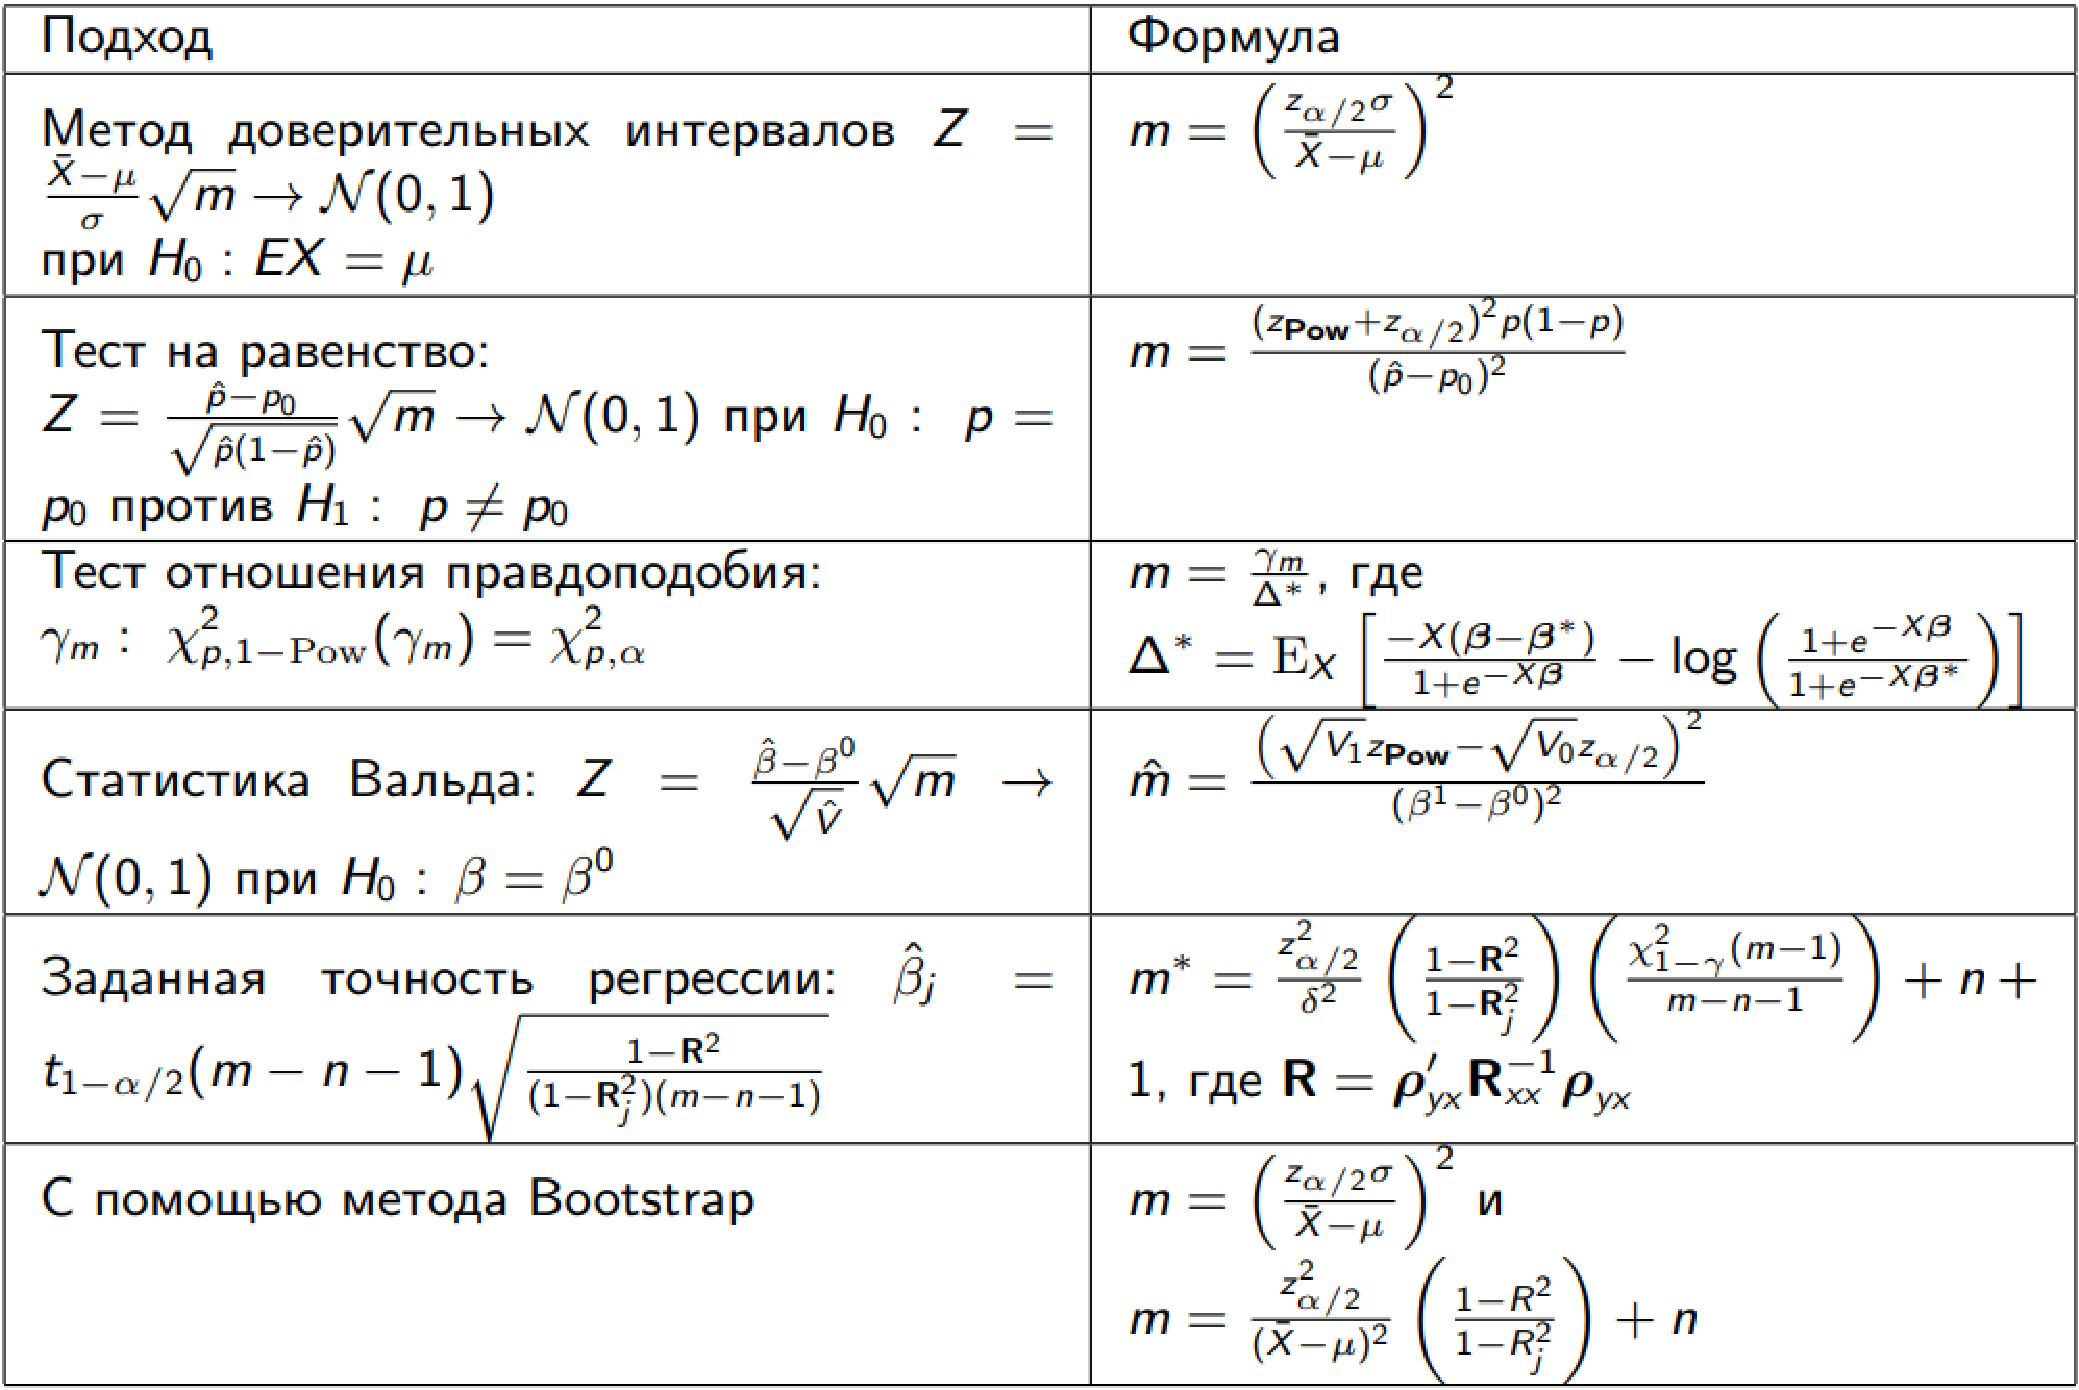
\includegraphics[scale=0.32]{../data/pics/methods.pdf}
\caption{}
\label{methods}
\end{figure}

\end{frame}

\begin{frame}
\frametitle{Постановка задачи раннего прогнозирования}
\begin{block}{Дано}
Выборка размера m: $~\mathfrak D = \{\textbf{x}_i, y_i\}_{i=1}^m,$

где $\textbf{x}_i \in \mathbb{R}^{n}$ - вектор признаков, $~y_i \in \mathbb{Y}$.
\end{block}

\begin{block}{Обобщённая линейная модель}
Зависимая переменная $y$ аппроксимируется обобщенной линейной моделью:
$$
\hat{y_i} = f(\mathbf{x}_i, \mathbf{w}) = \mu(\mathbf{w}^{\top}\mathbf{x}_i),
$$
$$
 \mu = \text{id} \text{ --- задача регрессии},
$$
$$
\mu(\mathbf{w}^{\top}\mathbf{x}_i) = \frac{1}{1 + \exp(-\mathbf{w}^{\top}\mathbf{x}_i)} \text{ --- задача классификации}
$$
\end{block}



\end{frame}

\begin{frame}
\frametitle{Постановка задачи раннего прогнозирования}

\begin{block}{Функция ошибки $S(\mathbf{w}, \mathfrak{D})$ для задач регрессии и классификации}
$$
S_{\text{reg}}(\textbf{w} | \mathfrak{D}) = \frac{1}{|\mathfrak{D}|}\sum\limits_{\mathbf{x}, y \in \mathfrak{D}}(y - f(\mathbf{x}, \mathbf{w}))^2,
$$
$$
S_{\text{class}}(\textbf{w} | \mathfrak{D}) =  \frac{1}{|\mathfrak{D}|}\sum\limits_{\mathbf{x}, y \in \mathfrak{D}}\bigl(y\ln f(\mathbf{x}, \mathbf{w}) + (1 - y)\ln(1 - f(\mathbf{x}, \mathbf{w}))\bigr).
$$
\end{block}

\begin{block}{Функция ошибки}
Будем рассматривать ожидаемое значение функции $e^{-S(\hat{\mathbf{w}}(\mathfrak{D}_{\mathcal{L}}) | \mathfrak{D}_{\mathcal{T}}))}$ по разным обучающим и тестовым выборкам размера $m$:
$$
l(m) = \mathsf E e^{-S(\hat{\mathbf{w}}(\mathfrak{D}_{\mathcal{L}}) | \mathfrak{D}_{\mathcal{T}}))}.
$$
\end{block}

\end{frame}

\begin{frame}
\frametitle{Постановка задачи раннего прогнозирования}

\begin{block}{Функция правдоподобия}
Определим функцию правдоподобия и логарифмическую функцию правдоподобия выборки $\mathfrak D$:
$$
L(\mathfrak D, \textbf{w}) = \prod_{y, \textbf{x} \in \mathfrak D} p(y | \textbf{x}, \textbf{w}),~~~ l(\mathfrak D, \textbf w) = \sum_{y, \textbf{x} \in \mathfrak D_m}\log p(y | \textbf{x}, \textbf{w}),
$$
где $p(y | \textbf{x}, \textbf{w})$ ---  плотность зависимой переменной.
\end{block}

\begin{block}{Оценка вектора параметров и оптимальный набор признаков}
Для получения оптимального набора признаков и оценки $\hat{\mathbf{w}}$ используется принцип максимума правдоподобия:
$$
\hat{\textbf{w}}, \hat{\mathcal{A}} = \argmax_{\mathbf{w} \in \mathbb{W}, \mathcal{A} \subseteq \mathcal{J}} L(\textbf{w}_{\mathcal{A}} | \mathfrak D_{\mathcal{A}}) = \argmax_{\mathbf{w} \in \mathbb{W}, \mathcal{A} \subseteq \mathcal{J}} e^{-S(\textbf{w}_{\mathcal{A}} | \mathfrak D_{\mathcal{A}})},
$$
где $\mathcal{J} = \{1, 2, ..., n\}$ --- множество индексов.
\end{block}

\end{frame}

\begin{frame}
\frametitle{Постановка задачи раннего прогнозирования}
\begin{block}{Функция ошибки $l(m)$}
$\hat{l}(m)$ --- оценка функции $l(m)$, посчитанная с помощью метода бутстреп по разным обучающим и тестовым подвыборкам размера $m$ выборки $\mathfrak{D}$.
\end{block}

\begin{block}{Бутстреп}
Есть 2 варианта генерации подвыборок:
\begin{itemize}
		\item $\mathfrak D^{\prime} \sim \mathcal{U}(\mathfrak{D})$ --- вариант 1, с полной информацией,
		\item $\mathfrak D^{\prime} \sim \mathcal{U}(\mathfrak{D}^0), \mathfrak{D}^0 \subset \mathfrak{D}, |\mathfrak{D}^0| = m^{\prime}$ --- вариант 2, с неполной информацией.
\end{itemize}
\end{block}
\end{frame}

\begin{frame}
\frametitle{Предлагаемый метод решения}

\begin{block}{Семейство функций $\Phi$}
Для предсказания значения функции $\hat{l}(m)$ при $m > m_0$ введем параметрическое семейство функций:
$$
\Phi = \{\phi(m) =  a + b\cdot e^{c \cdot m} ~|~ a, b \in \mathbb{R}, c \in (-\infty, 0)\}.
$$
\end{block}

\begin{block}{Аппроксимация $\phi(m) \sim \hat{l}(m)$}
Аппроксимация функции  $\hat{l}(m)$ является решением следующей задачи:
$$
\hat{\phi} =  \argmin_{\phi \in \Phi}\text{MAE}(\hat{l}, \phi, 1, m_0),
$$
где
$$
\text{MAE}(\psi, \phi, m_1, m_2) = \frac{1}{m_2 - m_1 + 1}\sum_{i=m_1}^{m_2}|\phi(i) - \psi(i)|.
$$
\end{block}

\end{frame}

\begin{frame}
\frametitle{Критерий достаточности объёма}

\begin{block}{Критерий достаточности объема}
Определим достаточный объем выборки $m^*$ как наименьший объём, что
$$
l(m^*) > (1 - \delta)\max\limits_{m^{\prime} > m^*}l(m^{\prime}),
$$
где $\delta$ --- достаточно малое пороговое значение.
\end{block}

\begin{block}{Оценка $\hat{m^*}$}
$\hat{m^*}$ --- наименьший объём выбрки, что
$$
\hat{\phi}(\hat{m^*}) > (1 - \delta)\max\limits_{m^{\prime} > \hat{m^*}}\hat{\phi}(m^{\prime}).
$$
\end{block}

\end{frame}

\begin{frame}
\frametitle{Вычислительный эксперимент}
\begin{block}{Цель эксперимента}
Проверить работоспособность предложенного метода.
\end{block}

\begin{block}{План эксперимента}
\begin{enumerate}
	\item Вычисление значимостей признаков, определение оптимальных наборов $\mathcal{A}(n^{\prime})$ размера $n^{\prime}$.
	\item Приближенное вычисление функции ошибки $\hat{l}(m)$ с помощью метода бутстреп, получение значения достаточного объёма выборки $m^*$.
	\item Построение модели аппроксимации функции ошибки  $\hat{l}(m)$ параметрическим семейством функций $\Phi$, получение аппроксимации функции ошибки $\hat{\phi}(m)$.
	\item Получение оценки достаточного объёма выборки $\hat{m^*}$.
\end{enumerate}
\end{block}

\end{frame}

\begin{frame}{Синтетические выборки}
Пусть $\mathbf{X} = [\boldsymbol{\chi}_1, ..., \boldsymbol{\chi}_n]$ --- набор векторов-столбцов.
\begin{figure}[h!t]\center
\centering\begin{tabular}{@{}c@{ }c@{ }c@{}}
\subfloat[Случайная выборка]{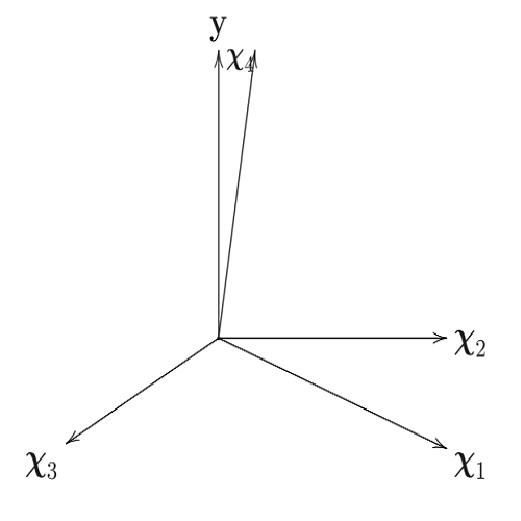
\includegraphics[width=0.5\textwidth]{../data/pics/random_sample.pdf}}&
\subfloat[Скоррелированная выборка]{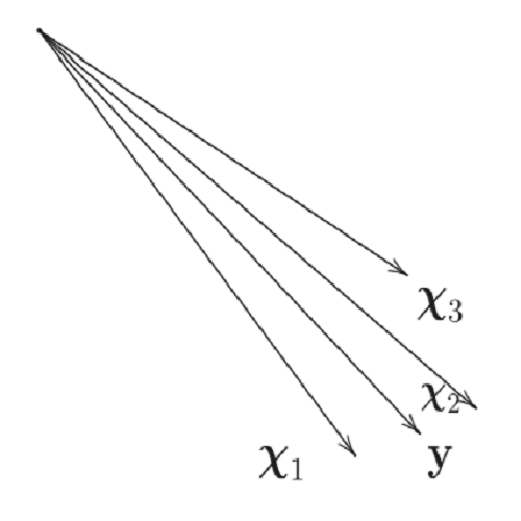
\includegraphics[width=0.5\textwidth]{../data/pics/correlated_sample.pdf}}\\
\end{tabular}
\centering
\caption{}
\label{fig01}
\end{figure}

\end{frame}

\begin{frame}{Синтетические выборки}

Пусть $\mathbf{X} = [\boldsymbol{\chi}_1, ..., \boldsymbol{\chi}_n]$ --- набор векторов-столбцов.

\begin{figure}[h!t]\center
\centering\begin{tabular}{@{}c@{ }c@{ }c@{}}
\subfloat[Ортогональная выборка]{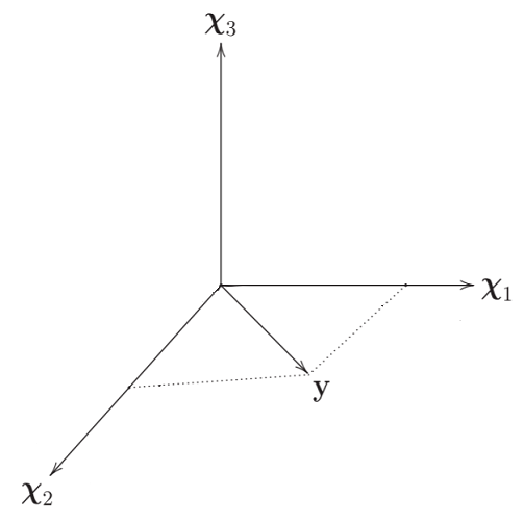
\includegraphics[width=0.5\textwidth]{../data/pics/orthogonal_sample.pdf}}&
\subfloat[Избыточная выборка]{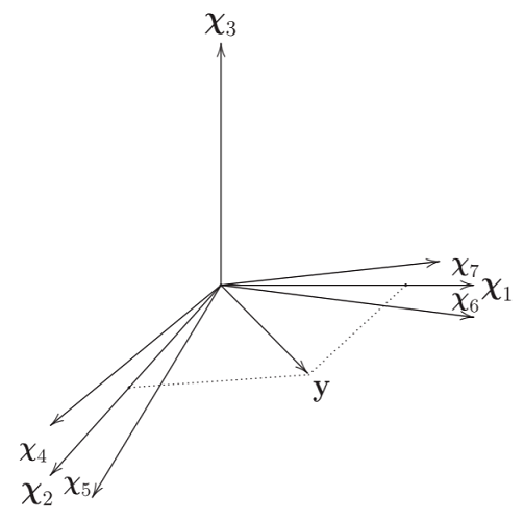
\includegraphics[width=0.5\textwidth]{../data/pics/redundant_sample.pdf}}\\
\end{tabular}
\centering
\caption{}
\label{fig01}
\end{figure}

\end{frame}


\begin{frame}
\frametitle{Синтетические выборки}

\begin{table}[h]
\begin{center}
\label{table1}
\begin{tabularx}{\textwidth}{|c|>{\centering\arraybackslash}X|>{\centering\arraybackslash}X|>{\centering\arraybackslash}X|>{\centering\arraybackslash}X|>{\centering\arraybackslash}X|}
\hline
	\centering Выборка & $m^*$ & $m$ & $n^*$ & $n$ & $\mathsf{D}\varepsilon$\\
	\hline
	Случайная выборка & 72 & 100 & 10 & 10 & 1\\
	\hline
	Скоррелированная выборка & 31 & 100 & 2 & 10 & 1\\
	\hline
	Ортогональная выборка & 45 & 100 & 10 & 10 & 0.5\\
	\hline
	Избыточная выборка & 22 & 100 & 5 & 10 & 0.5\\
\hline
\end{tabularx}
\end{center}
\end{table}

\end{frame}

\begin{frame}{Результаты эксперимента на синтетических выборках}

\begin{figure}[h!t]\center
\centering\begin{tabular}{@{}c@{ }c@{ }c@{}}
\textbf{Матожидание} & \textbf{Дисперсия}\\
\subfloat{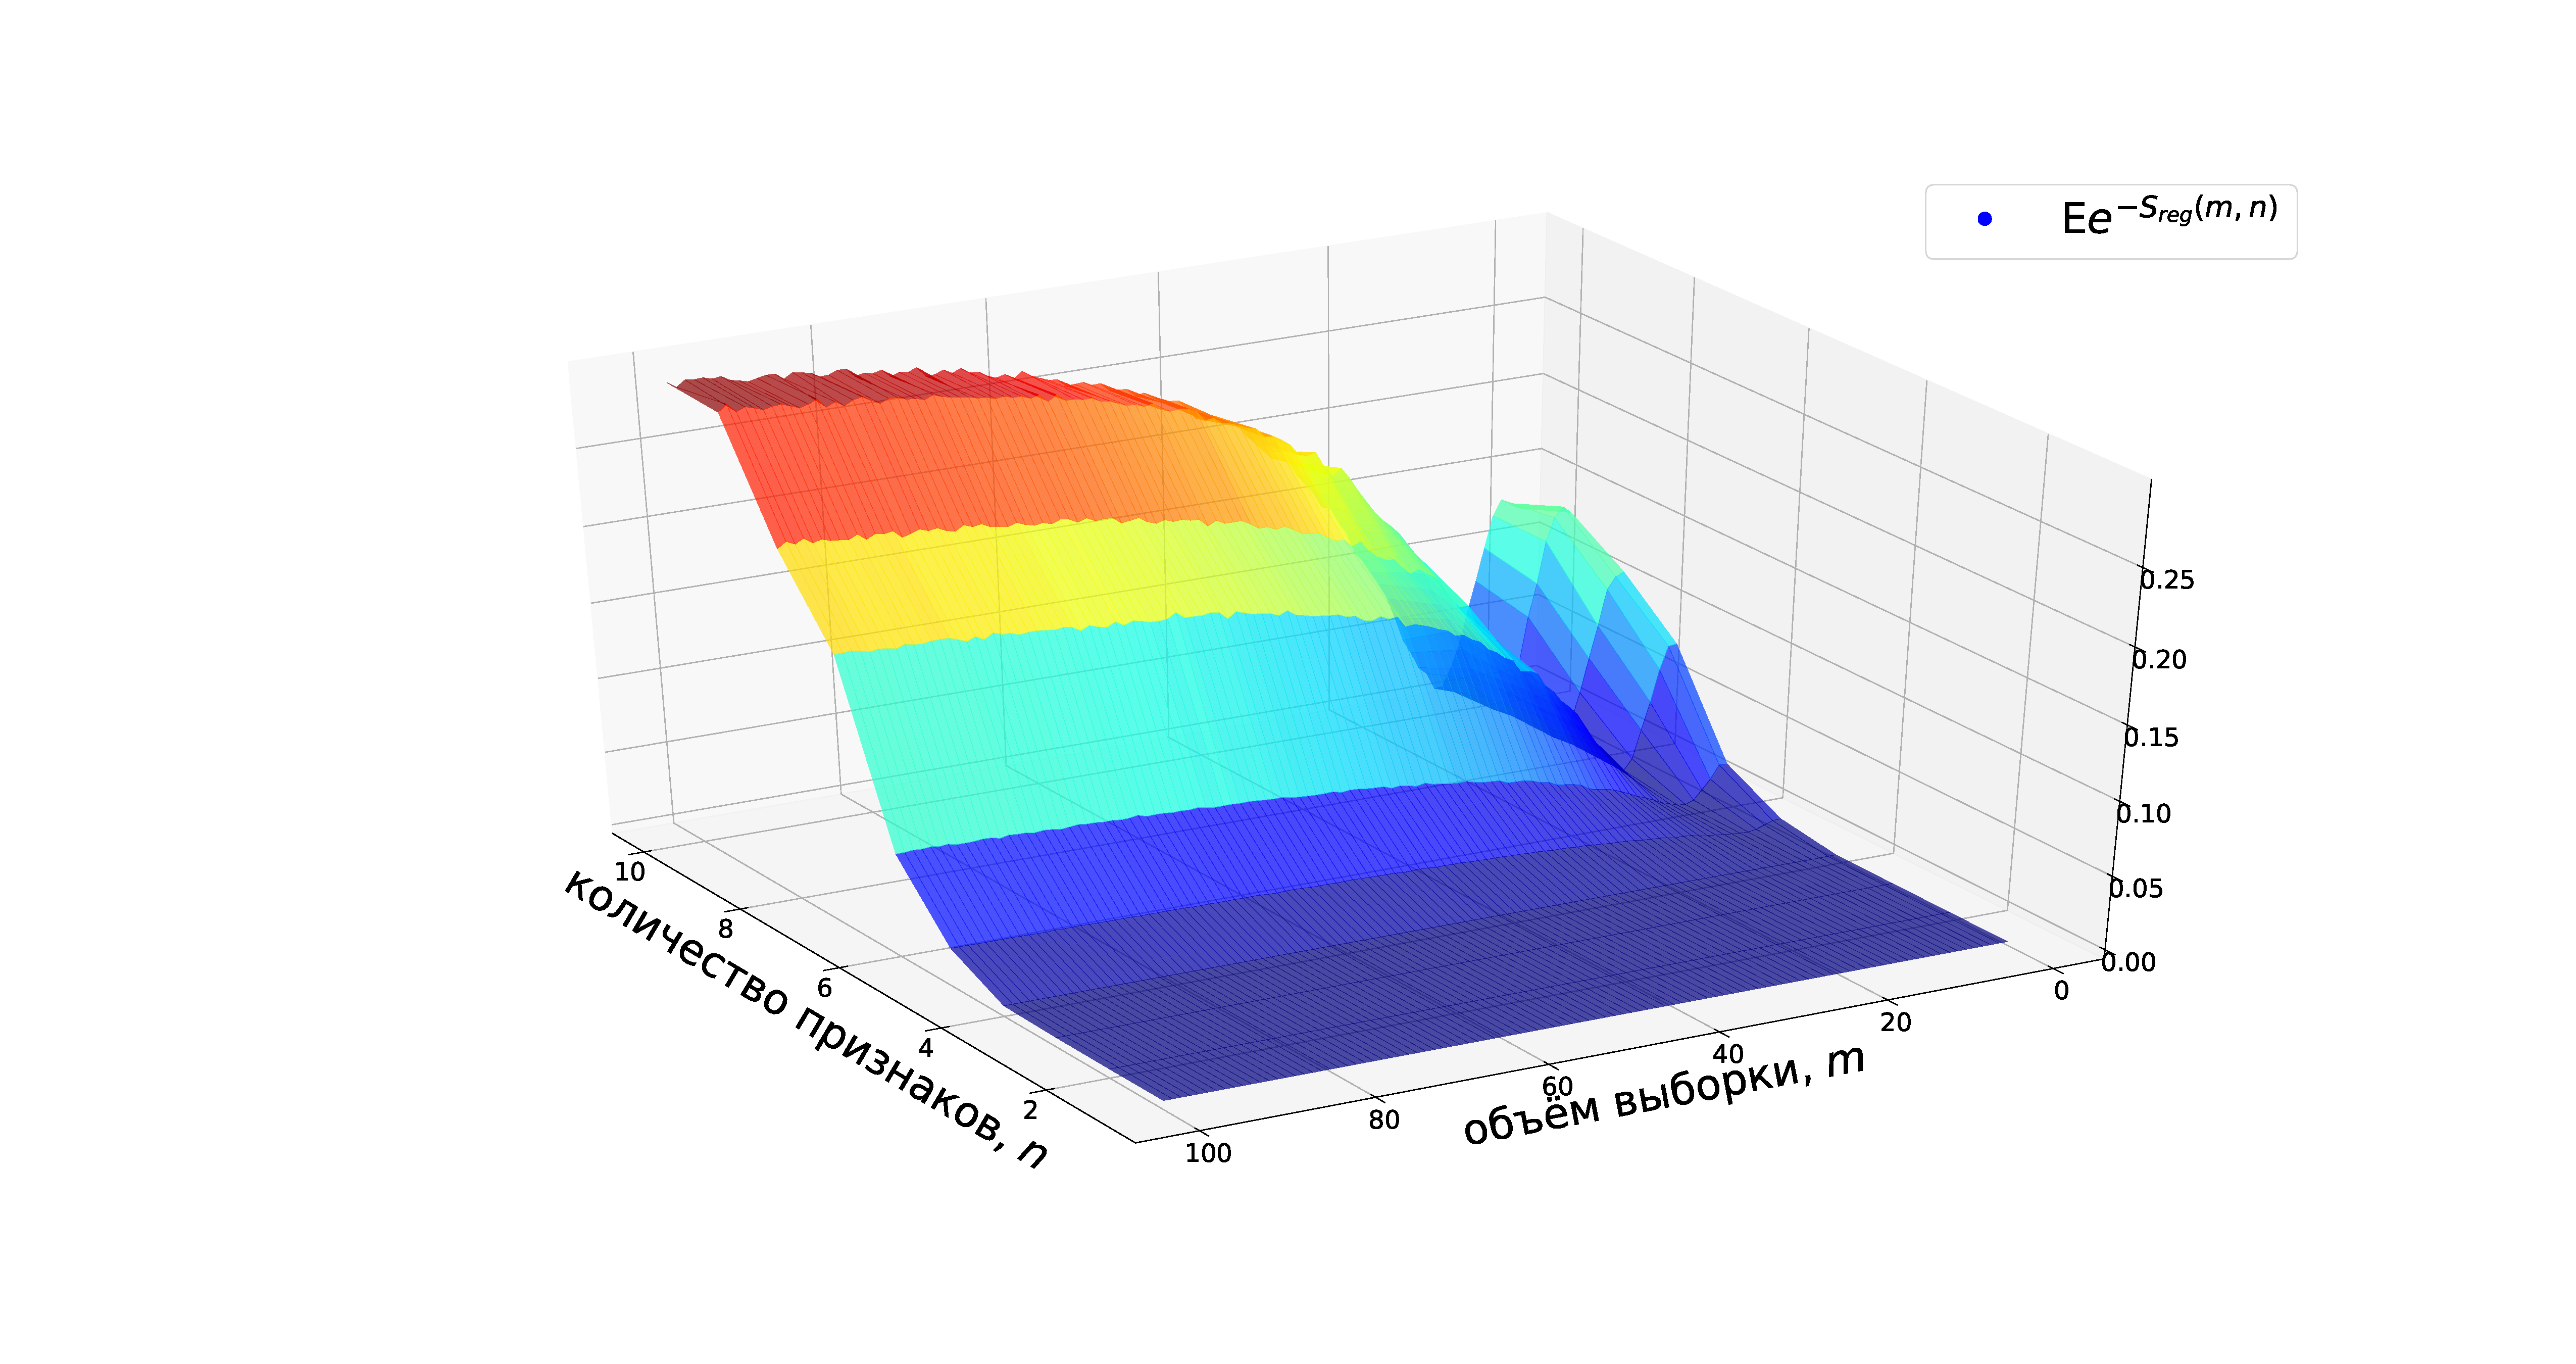
\includegraphics[width=0.55\textwidth]{../data/pics/adequate_random_sample_llh.pdf}}&
\subfloat{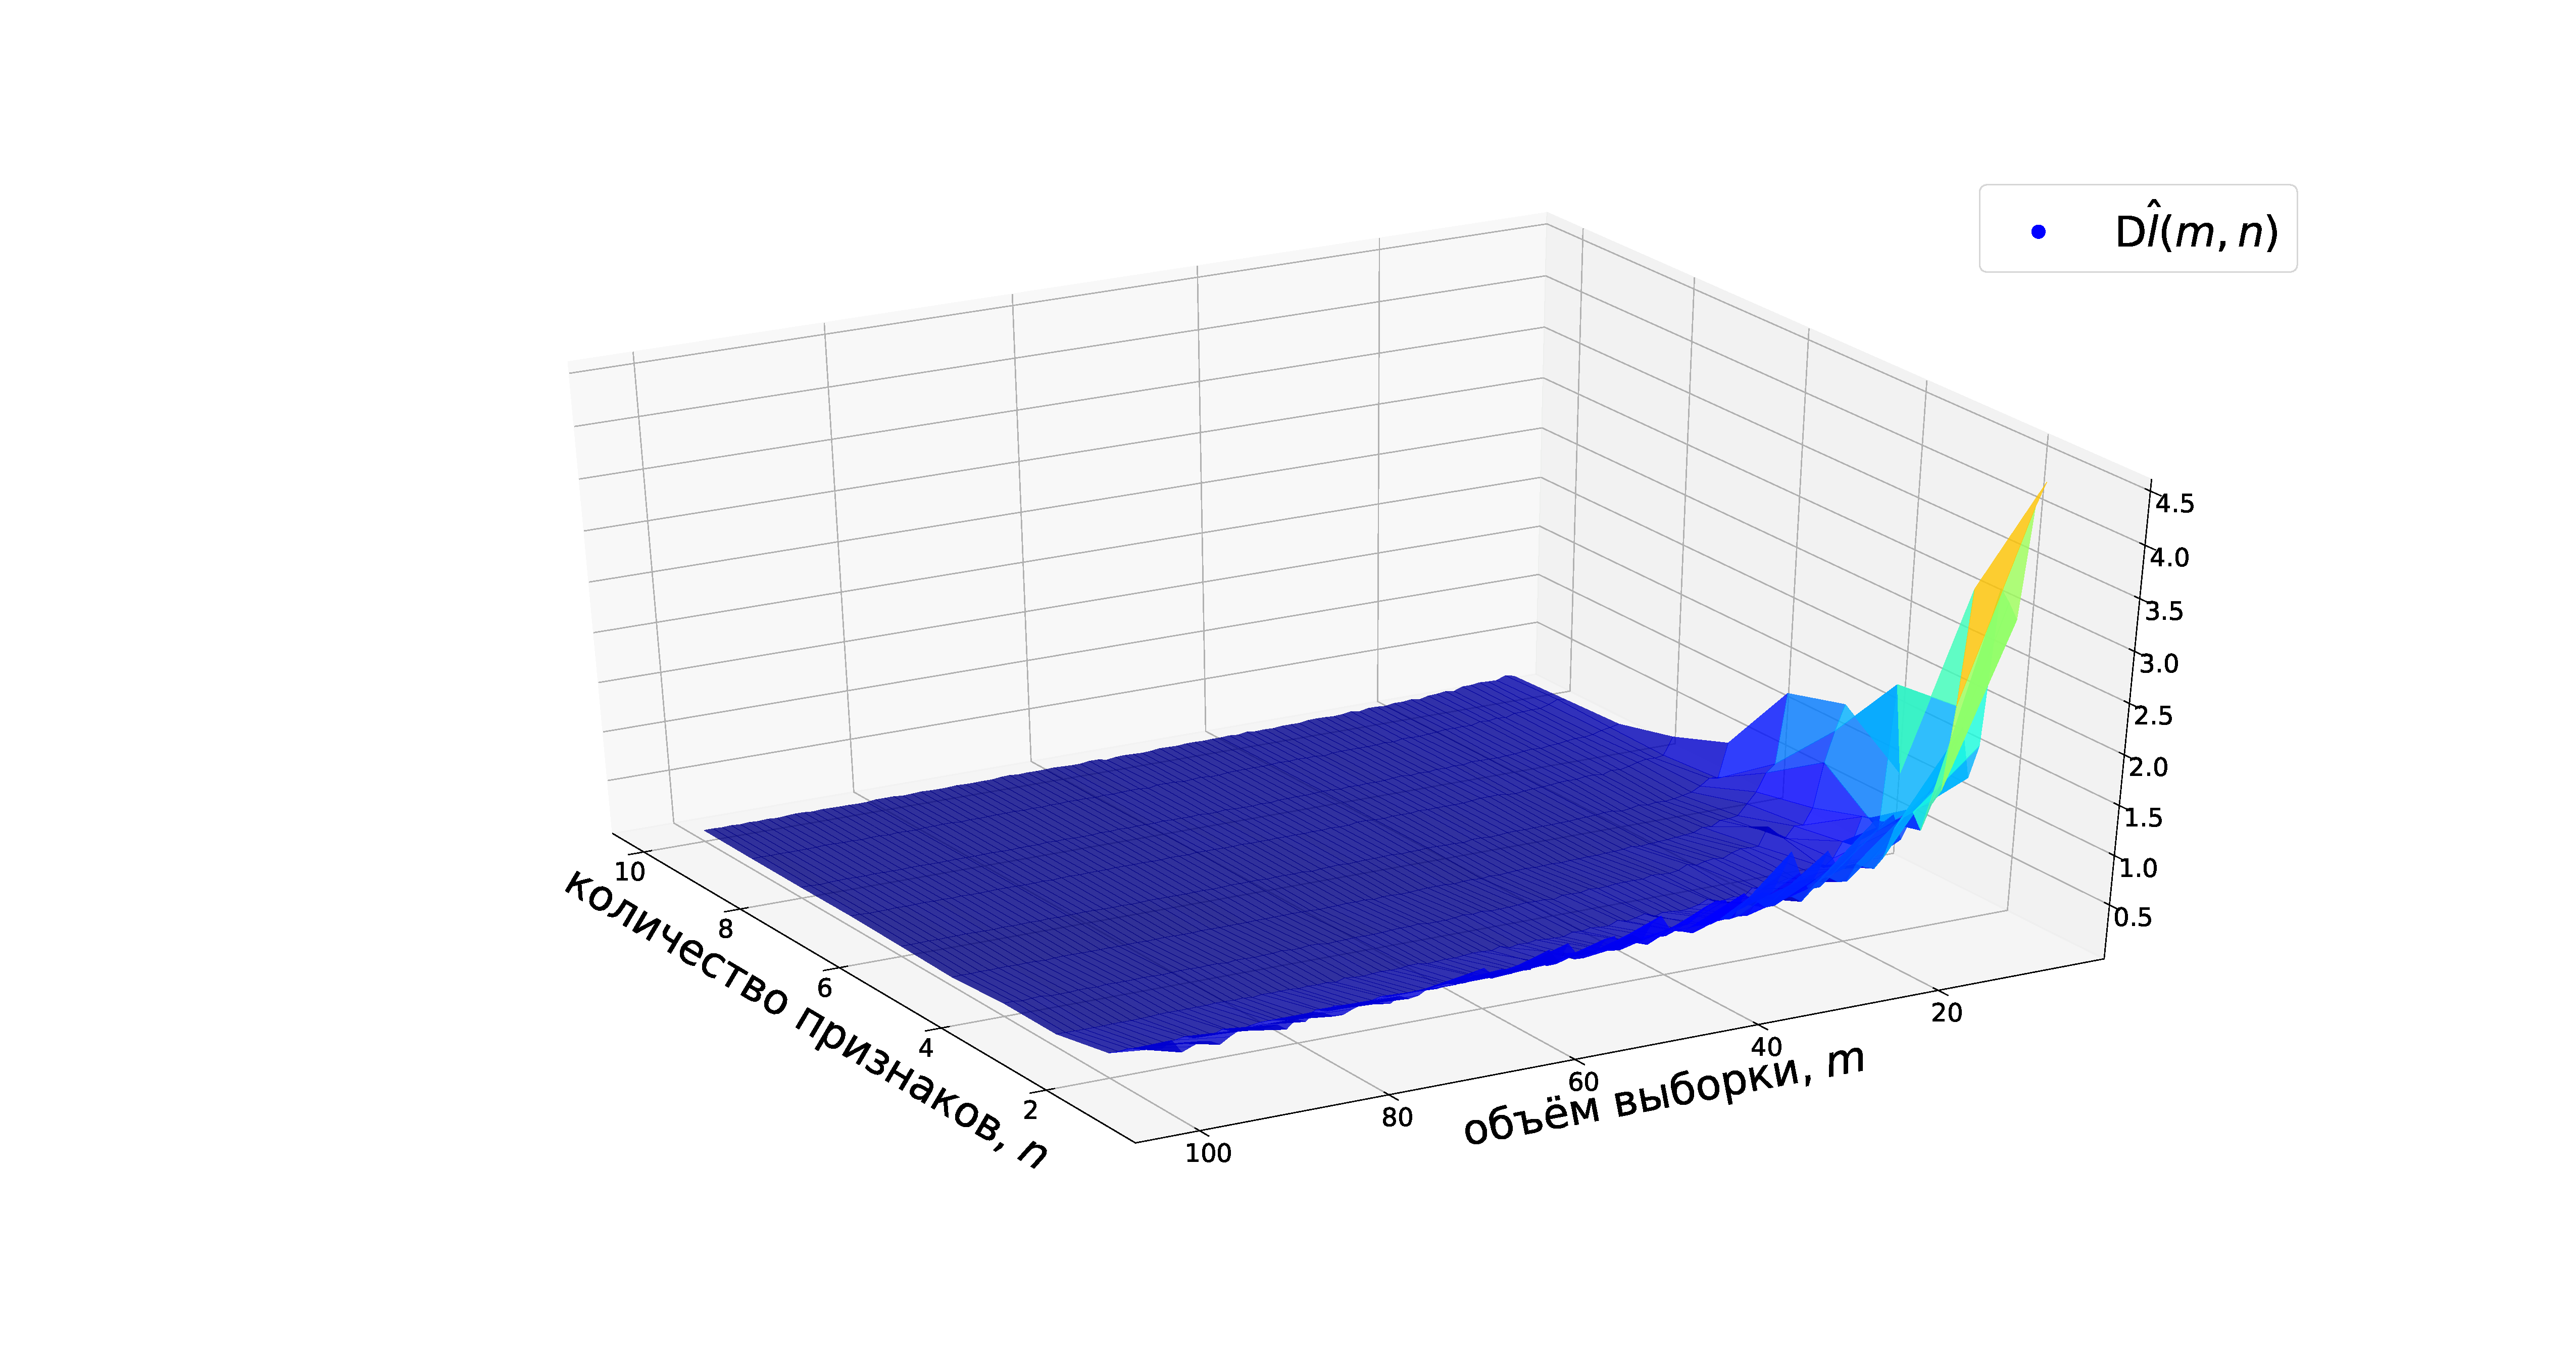
\includegraphics[width=0.55\textwidth]{../data/pics/adequate_random_sample_llh_std.pdf}}\\
\end{tabular}
\centering
\caption{Зависимость значения функции $e^{-S(m, n)}$ от объема выборки $m$ и количества параметров $n$ для случайной выборки}
\label{fig1}
\end{figure}

\end{frame}

\begin{frame}{Результаты эксперимента на синтетических выборках}

\begin{figure}[h!t]\center
\centering\begin{tabular}{@{}c@{ }c@{ }c@{}}
\textbf{Аппроксимация $e^{-S(m, n)}$} & \textbf{Предсказание $\hat{m^*}$}\\
\subfloat{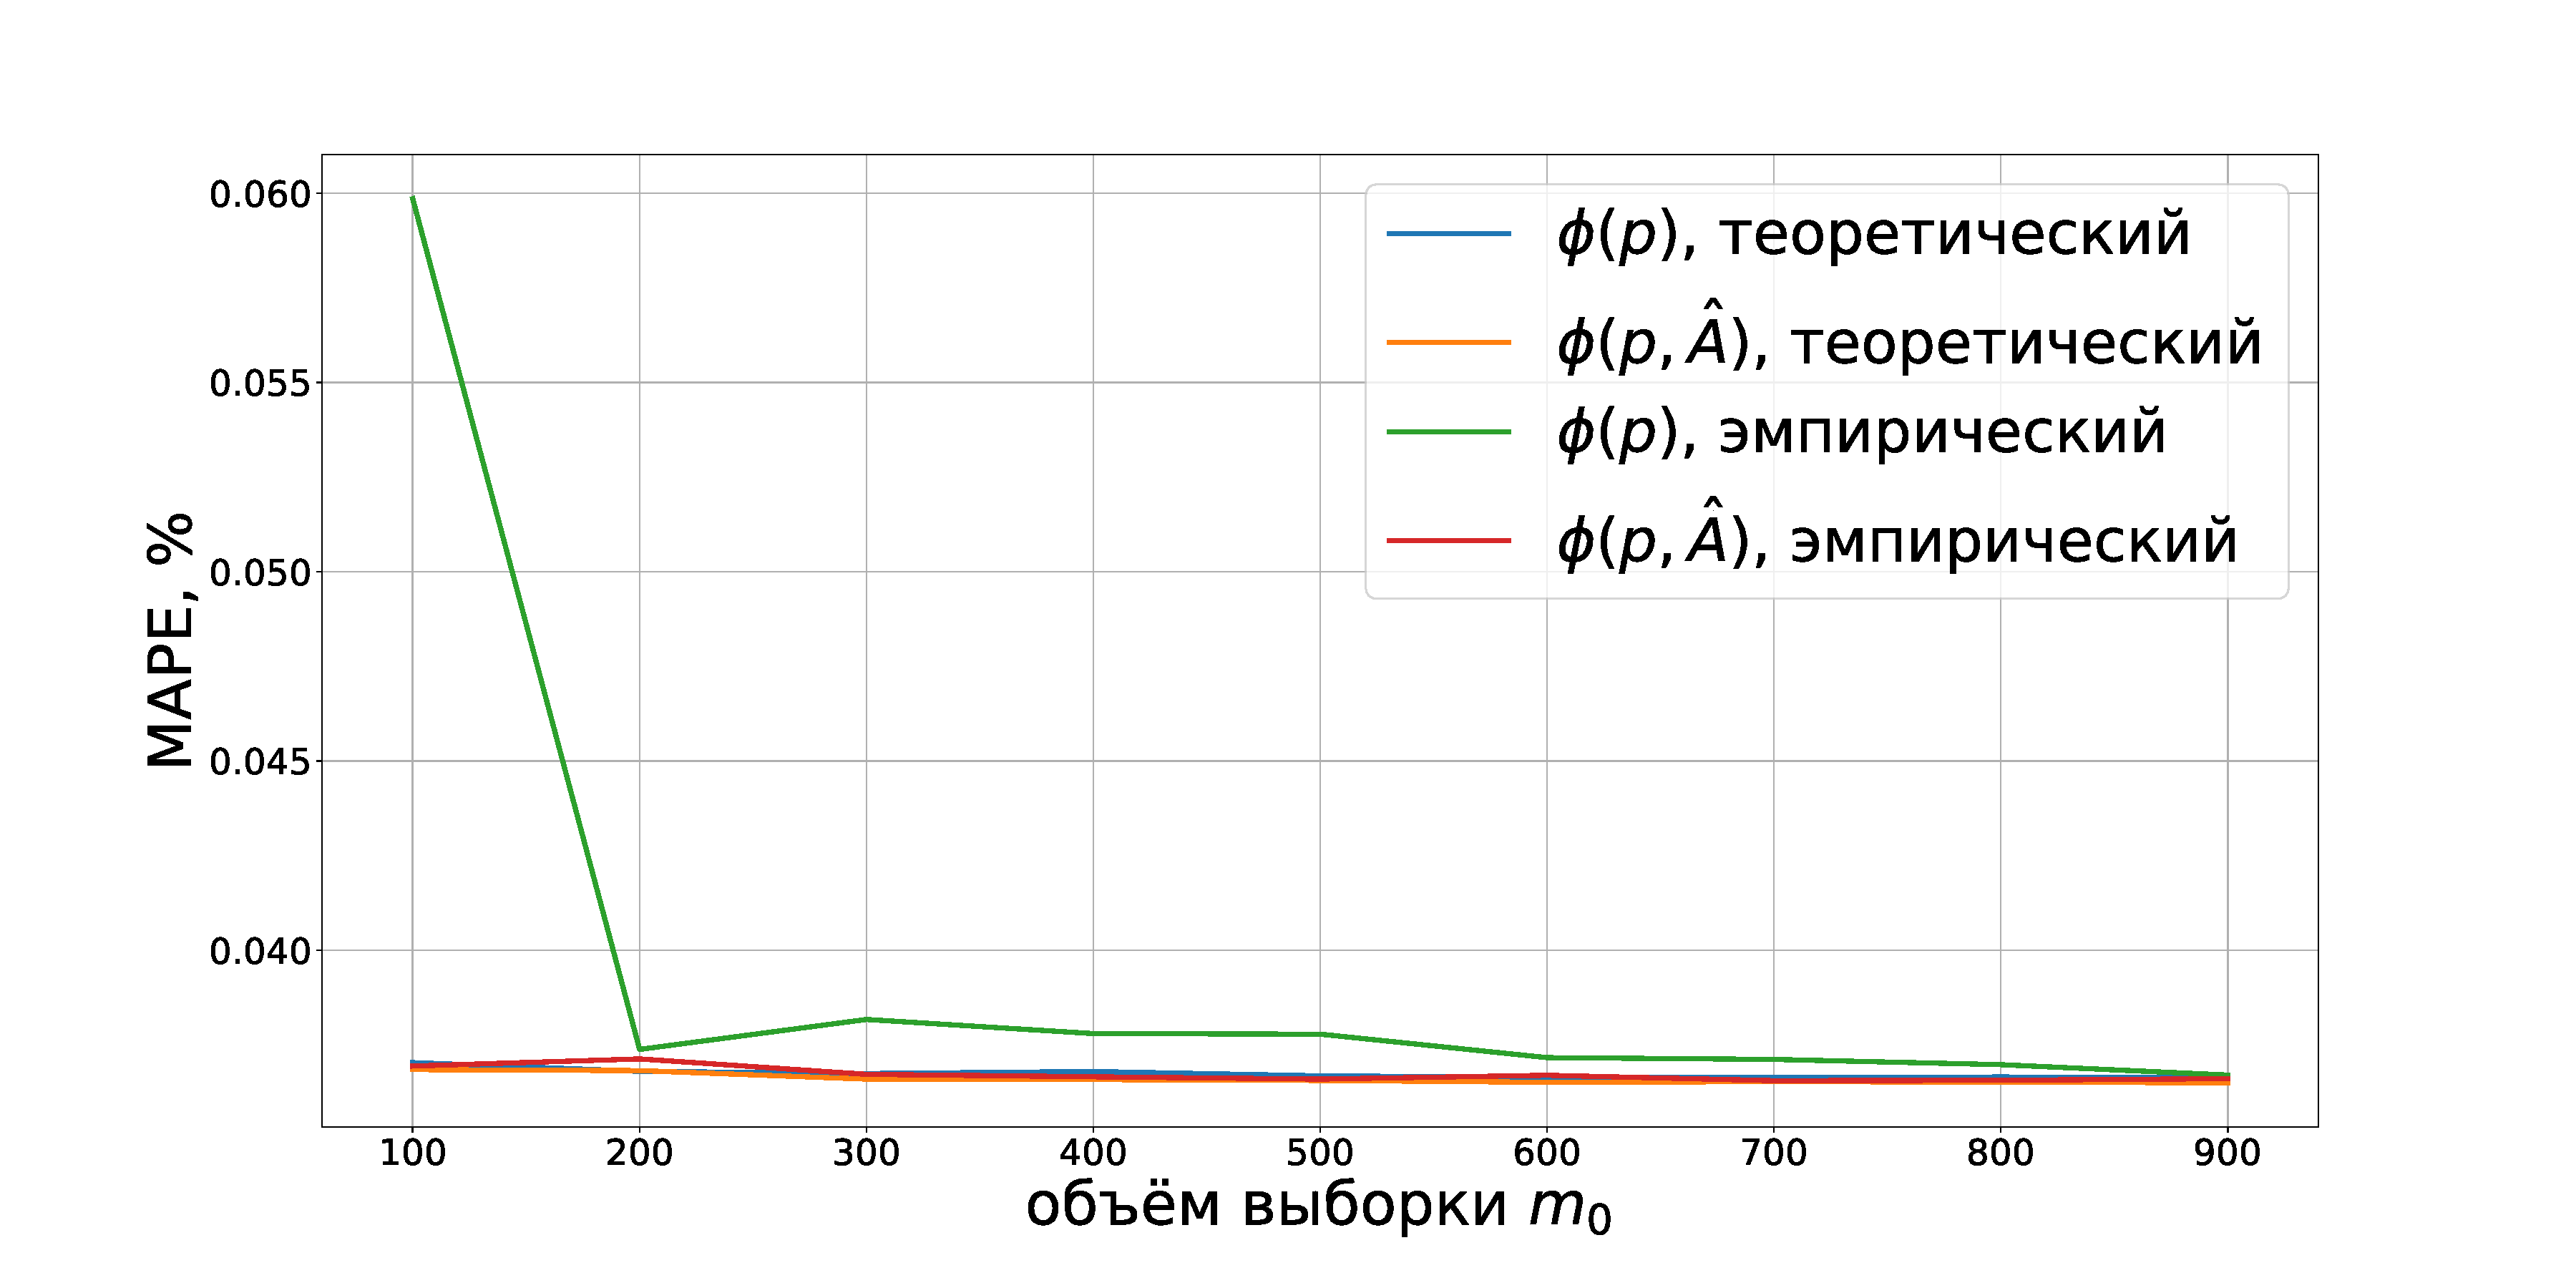
\includegraphics[width=0.55\textwidth]{../data/pics/adequate_random_sample_MAPE_comparison.pdf}}&
\subfloat{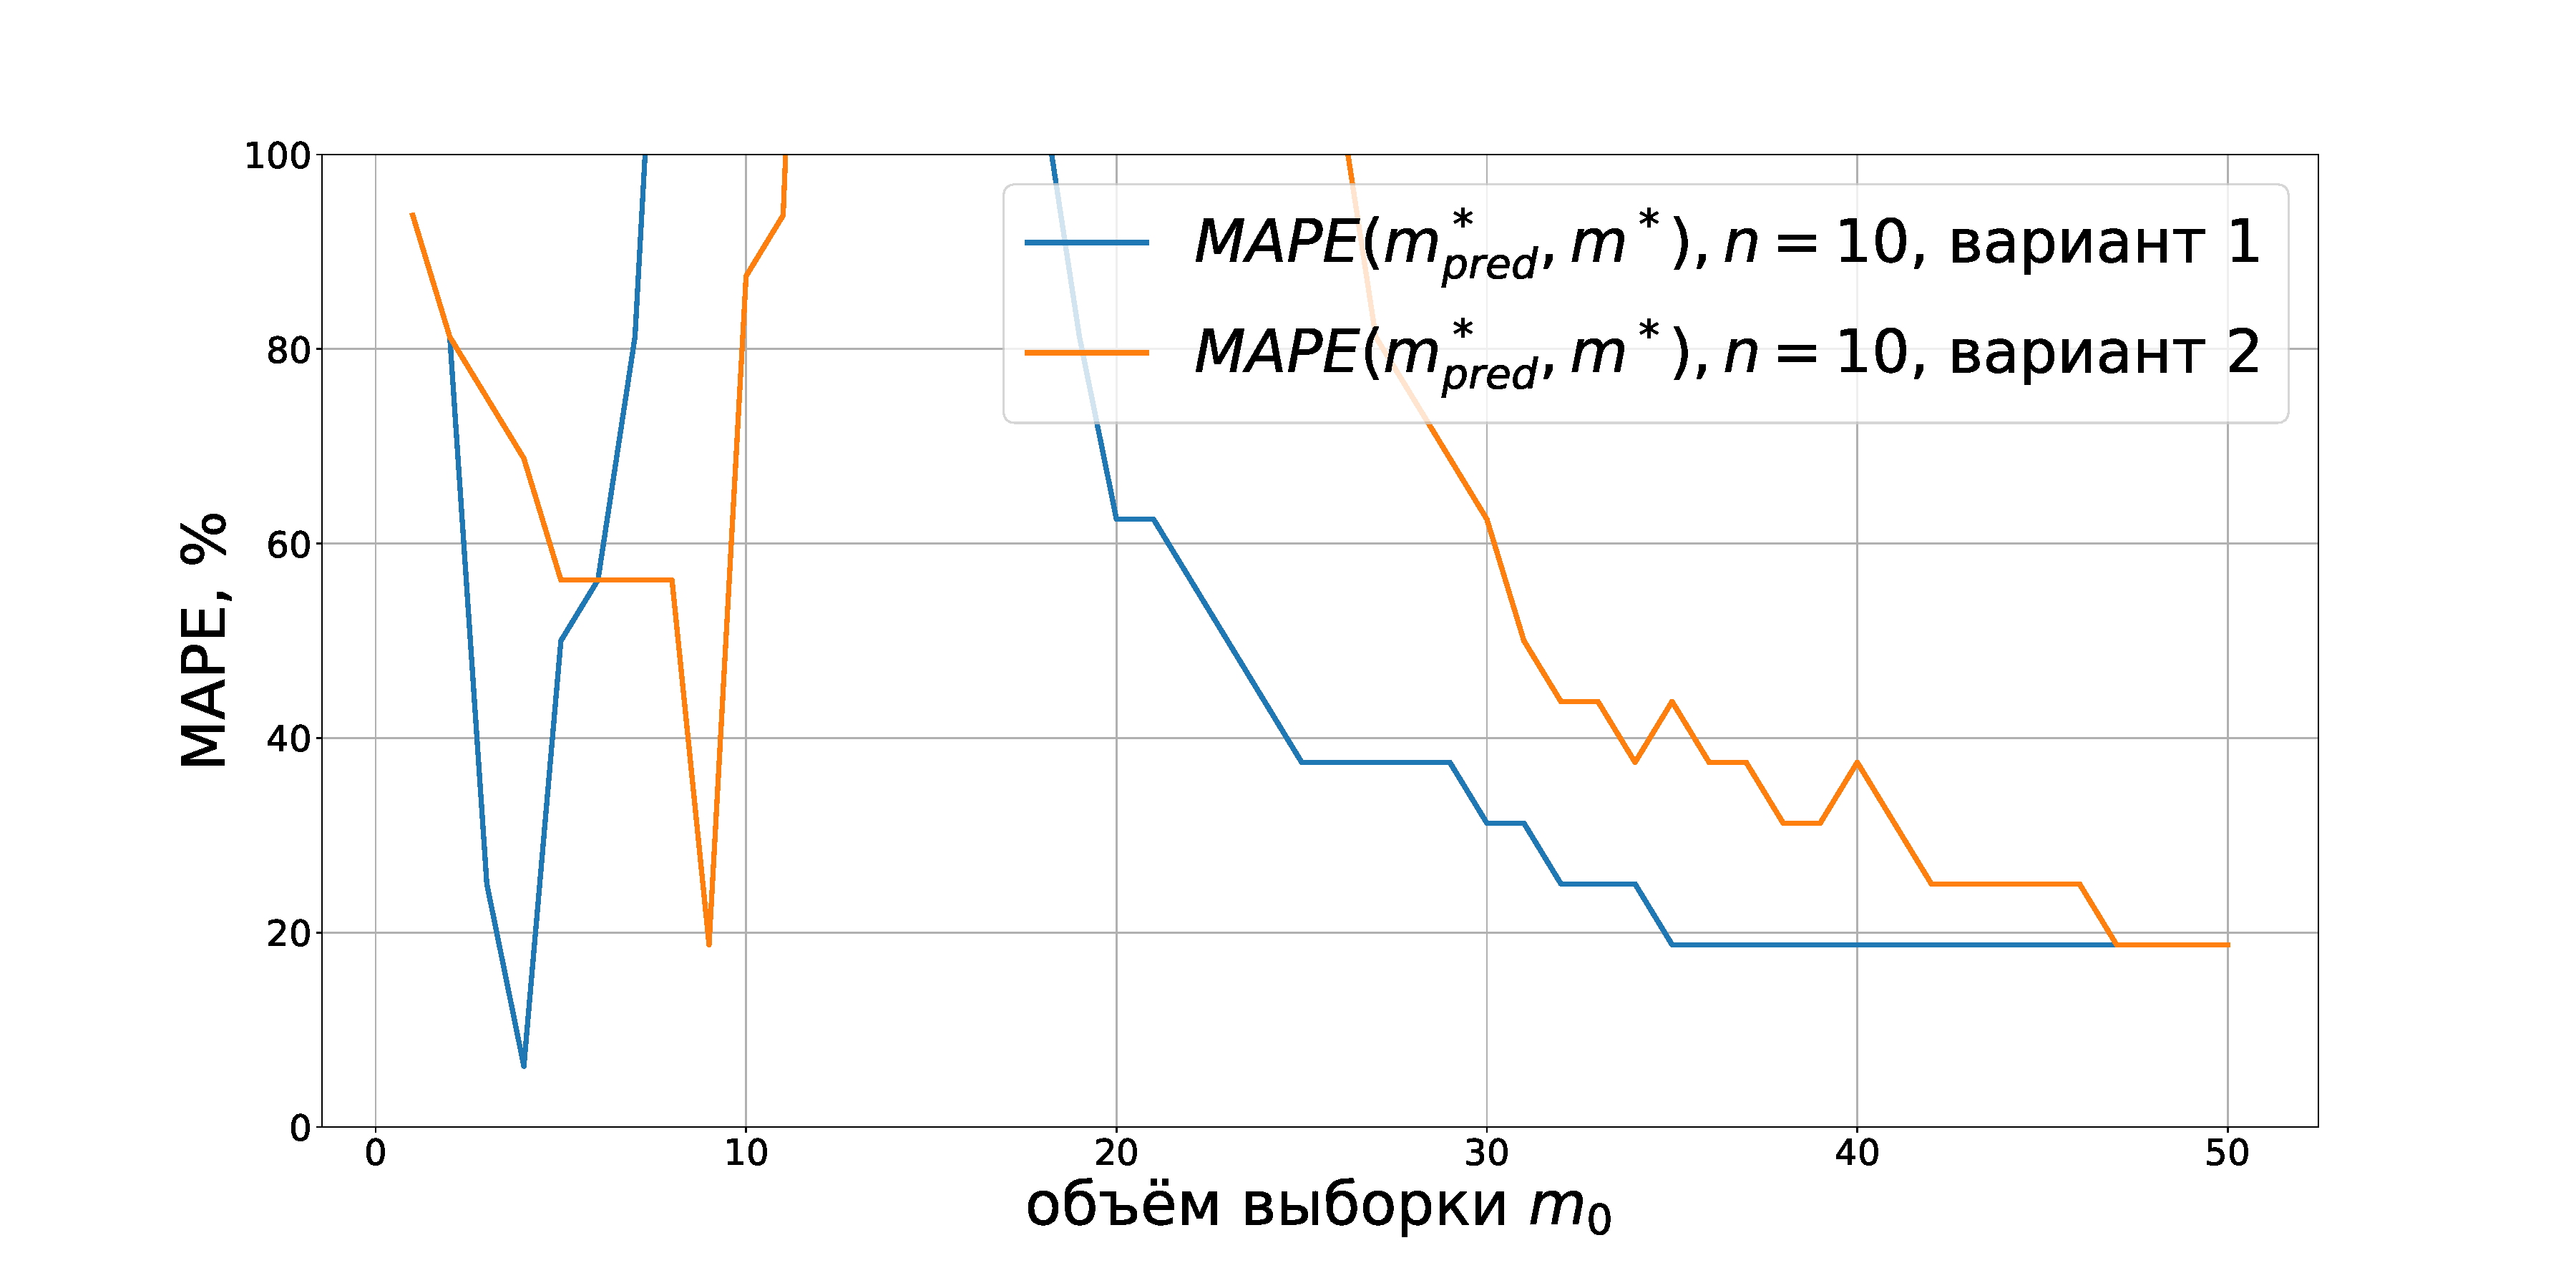
\includegraphics[width=0.55\textwidth]{../data/pics/adequate_random_sample_MAPE_m_comparison_n10.pdf}}\\
\end{tabular}

\caption{Качество предсказания $e^{-S(m, n)}$ и $m^*$ в зависимости от объема обучающей выборки $m_0$ для случайной конфигурации выборки}
\label{fig2}
\end{figure}

\end{frame}

\begin{frame}{Результаты эксперимента на синтетических выборках}

\begin{figure}[h!t]\center
\centering\begin{tabular}{@{}c@{ }c@{ }c@{}}
\textbf{Матожидание} & \textbf{Дисперсия}\\
\subfloat{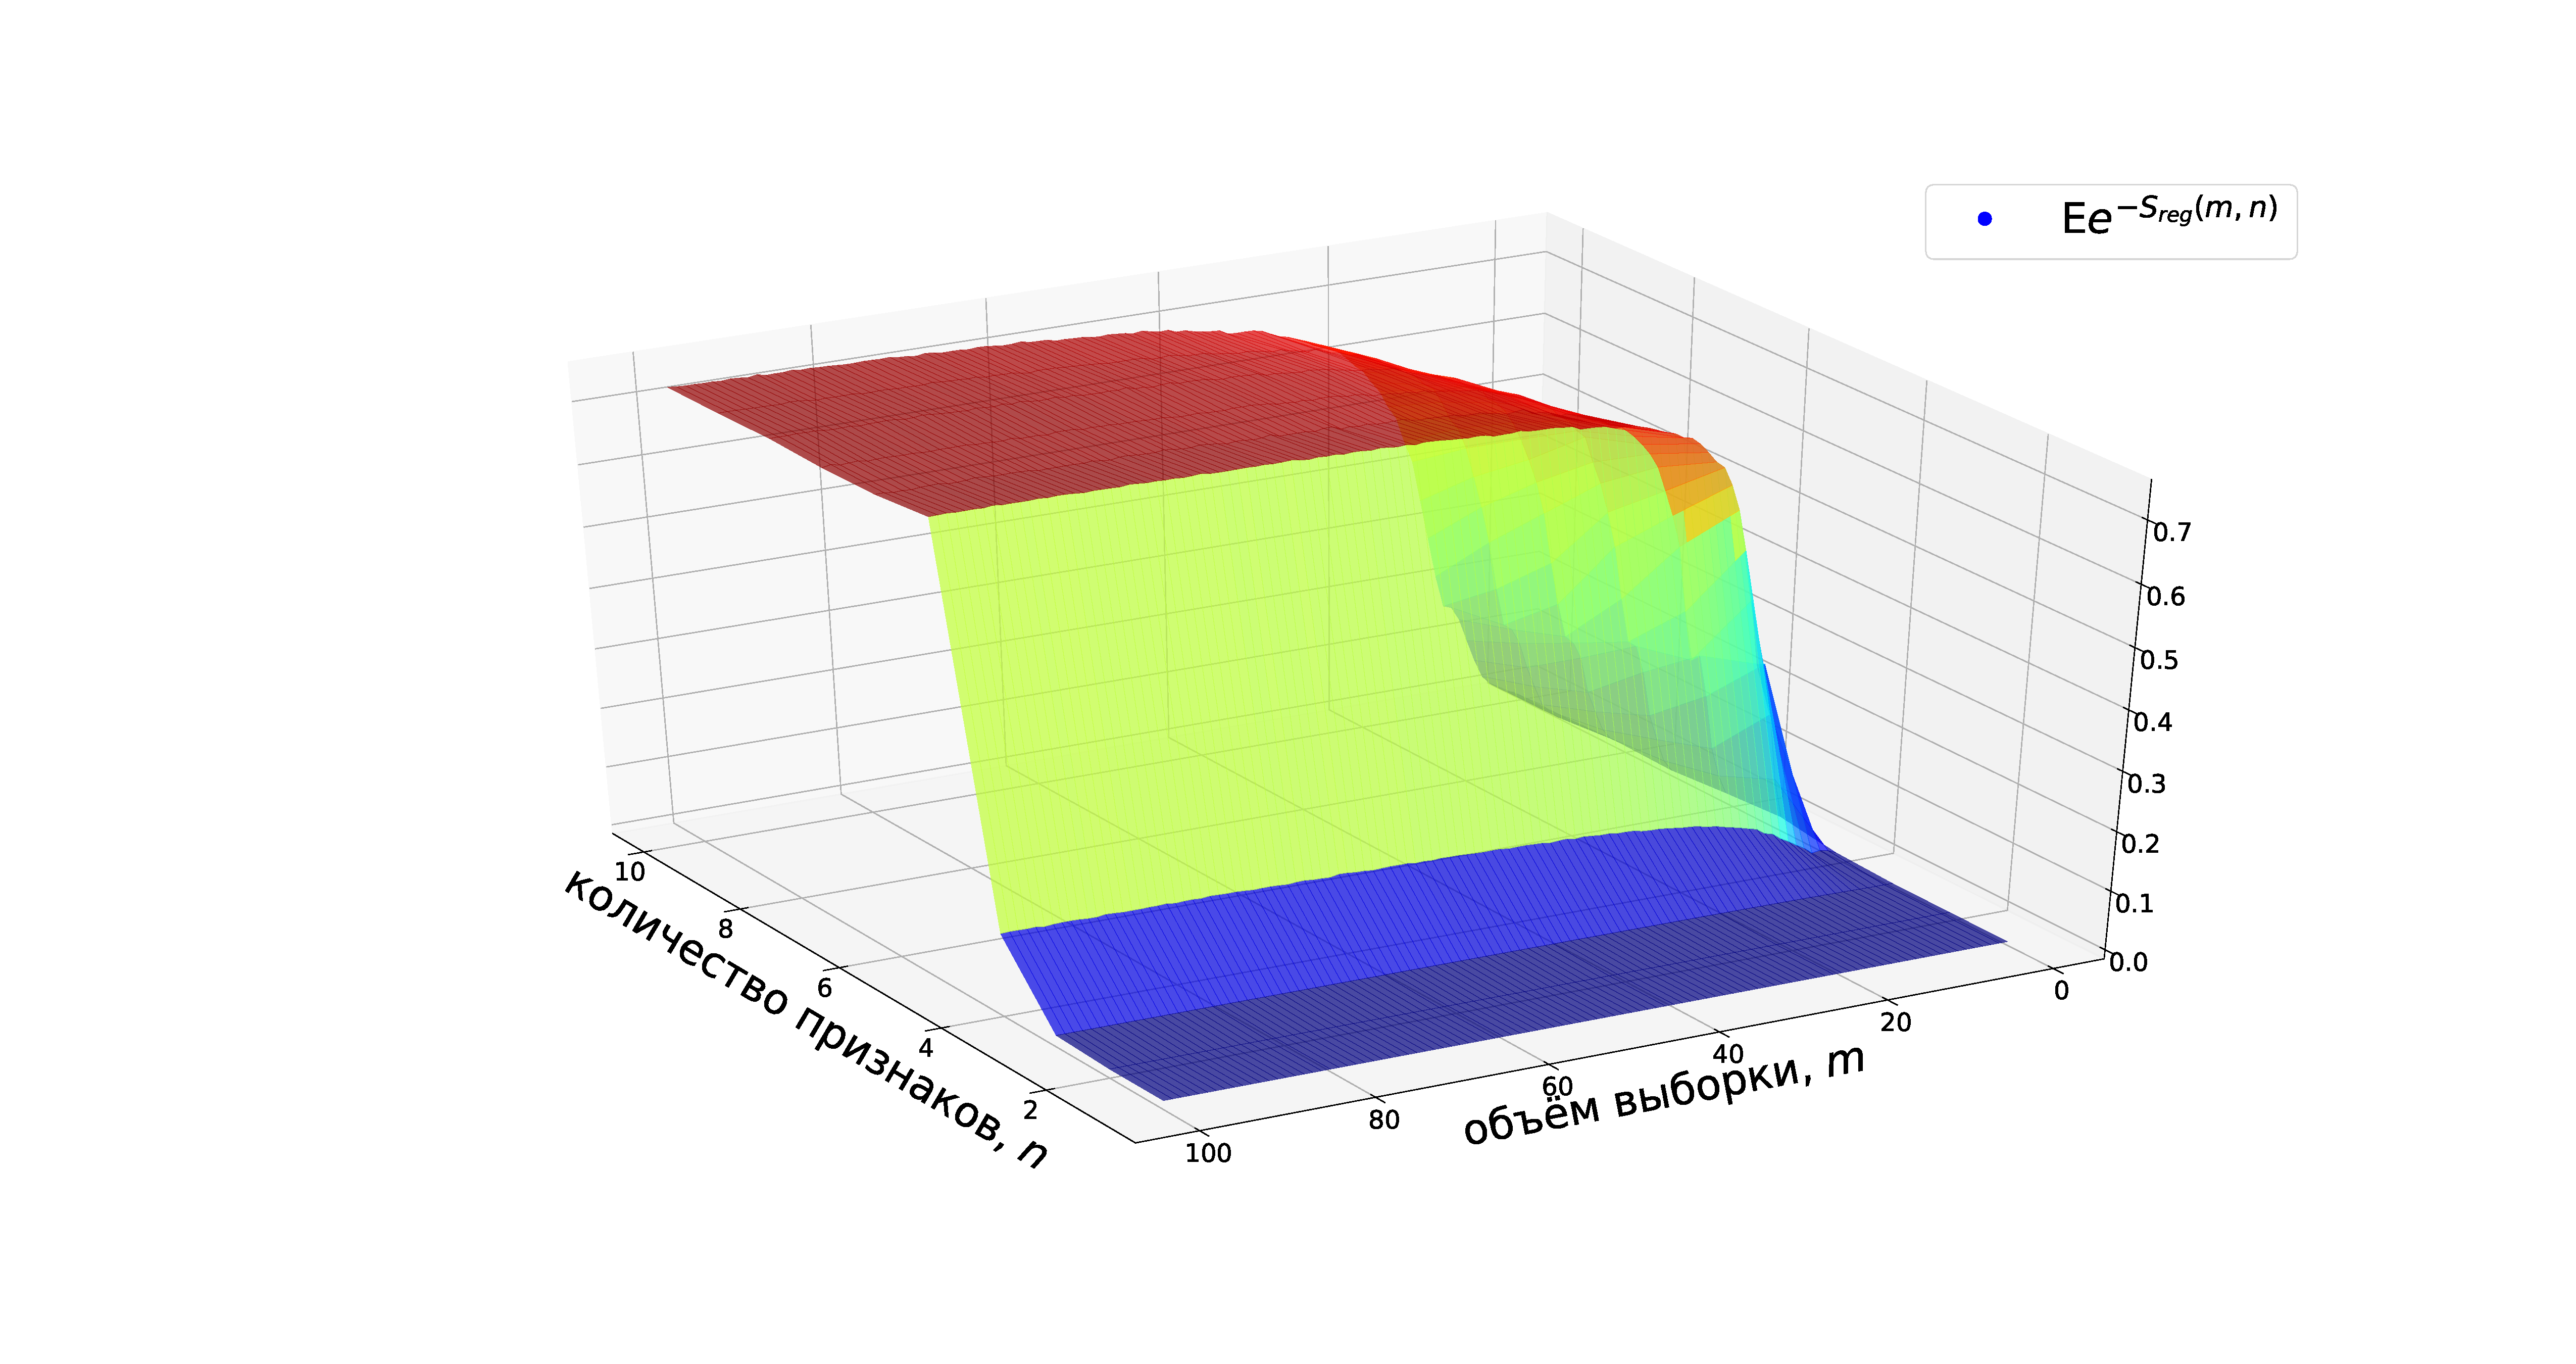
\includegraphics[width=0.5\textwidth]{../data/pics/adequate_redundant_sample_llh.pdf}}&
\subfloat{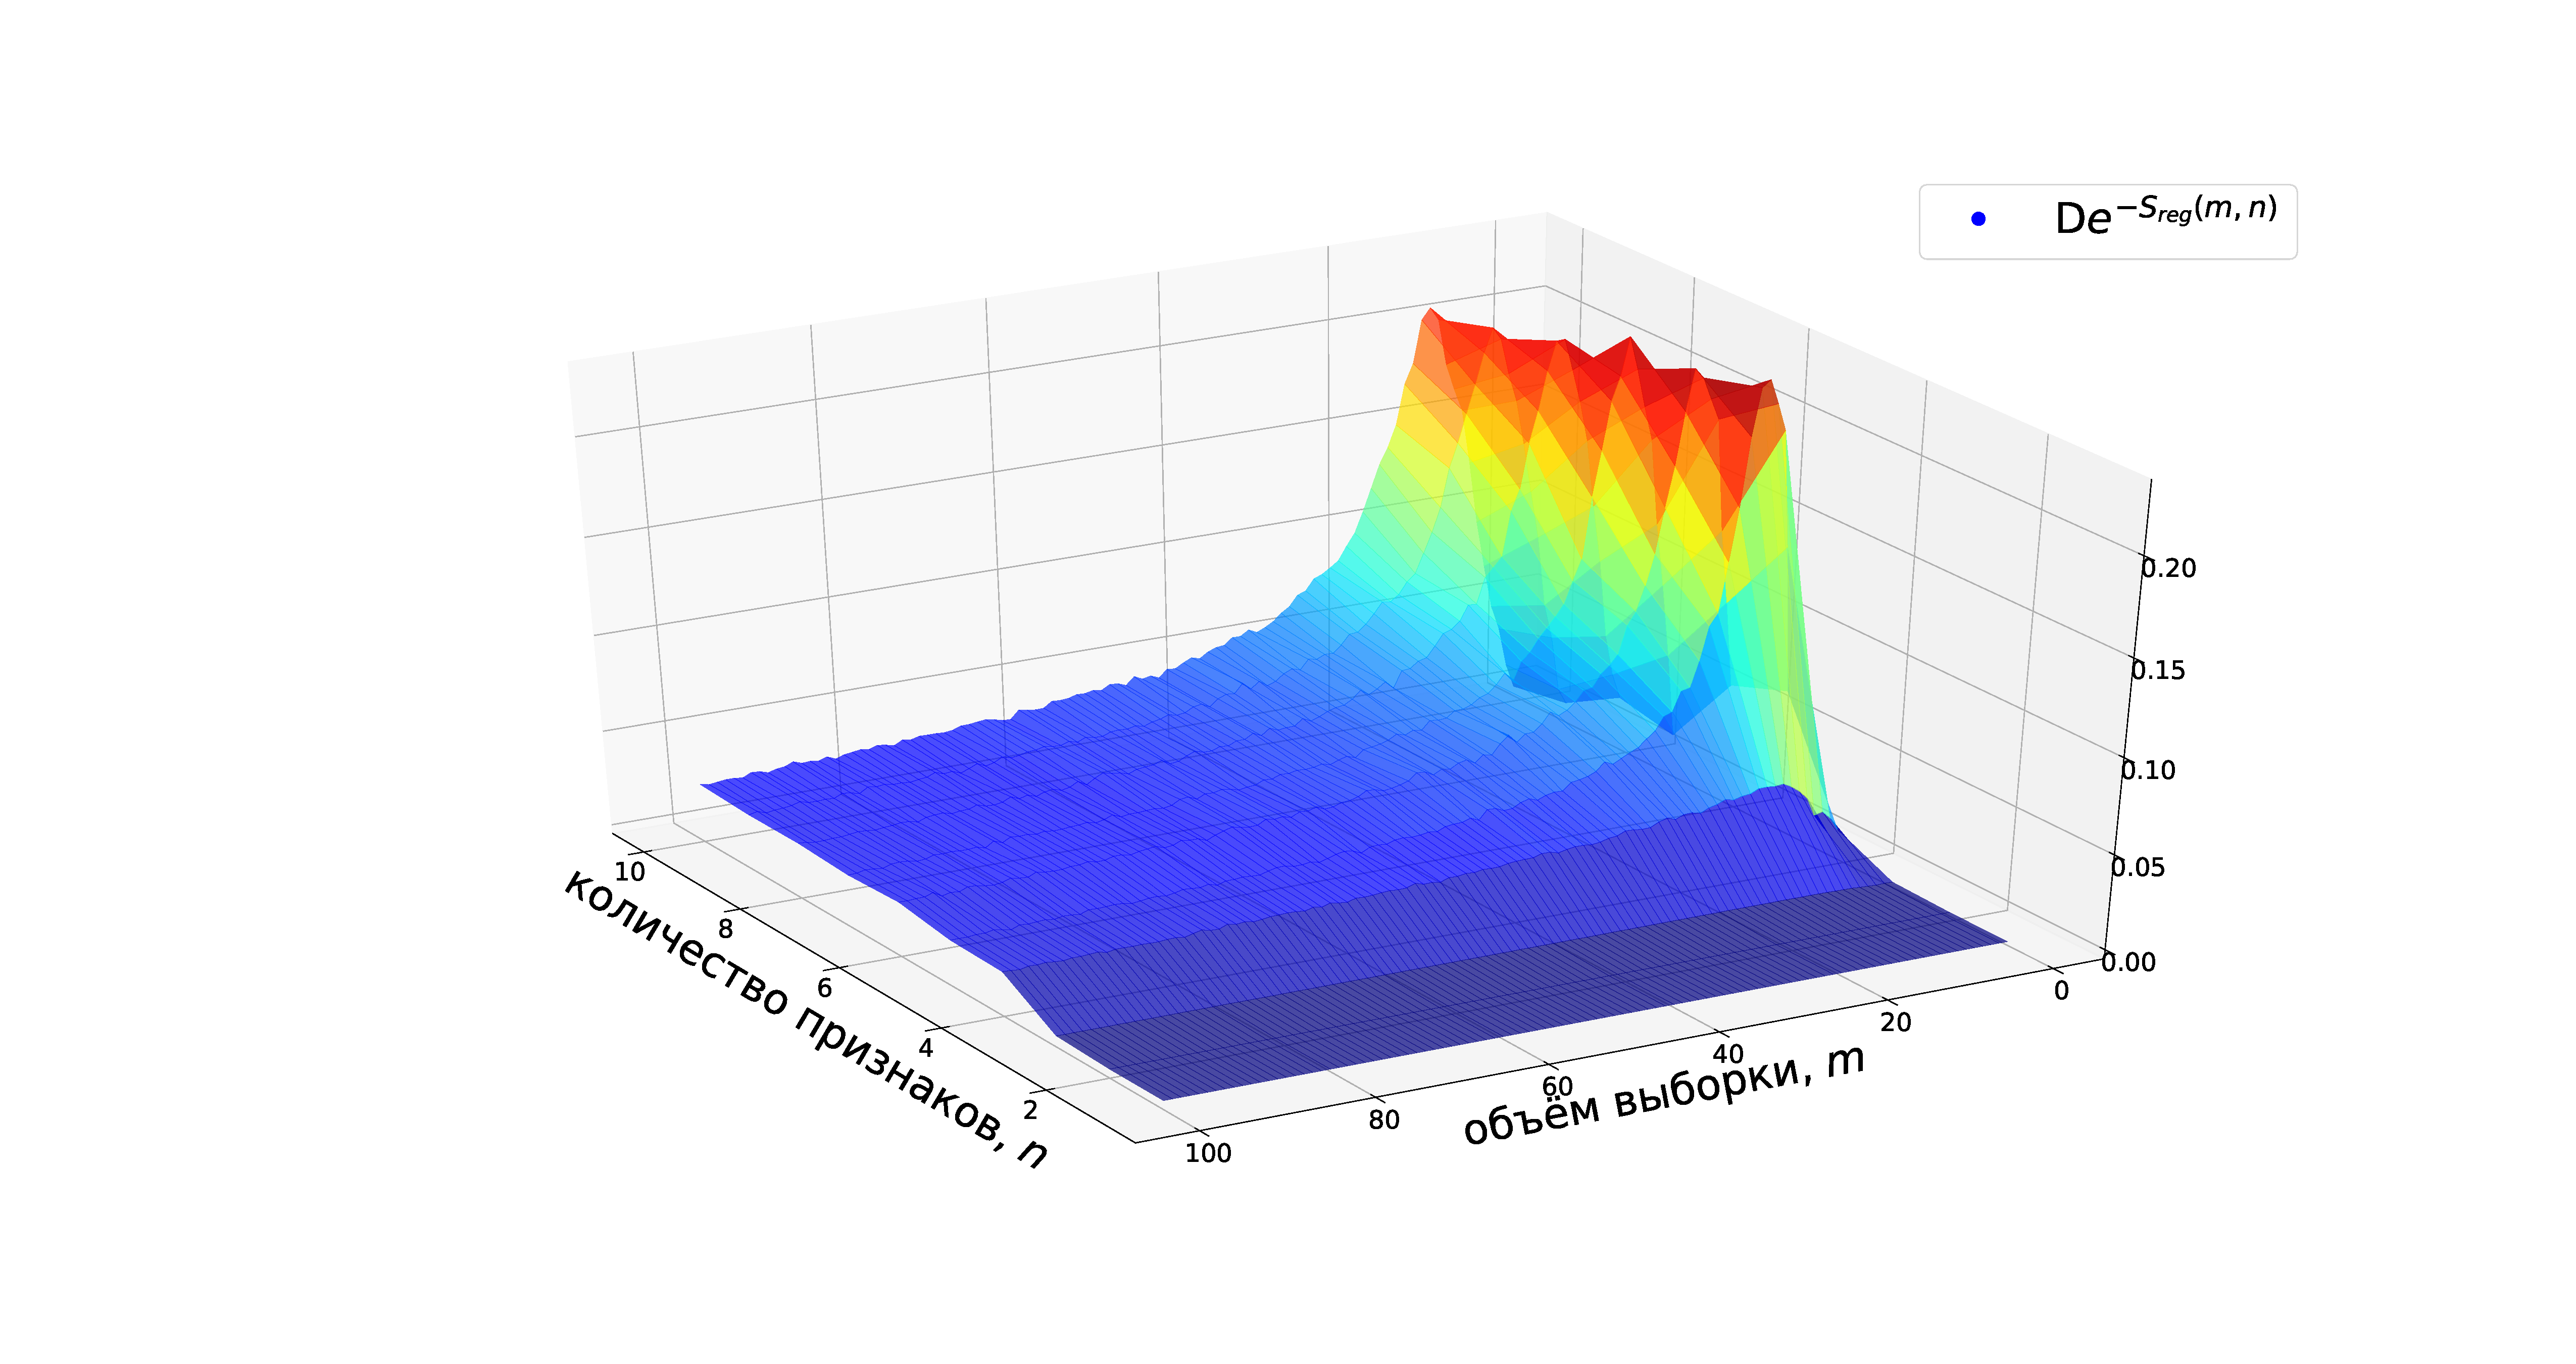
\includegraphics[width=0.5\textwidth]{../data/pics/adequate_redundant_sample_llh_std.pdf}}\\
\end{tabular}
\centering
\caption{Зависимость значения функции $e^{-S(m, n)}$ от объема выборки $m$ и количества параметров $n$ для случайной выборки}
\label{fig1}
\end{figure}

\end{frame}

\begin{frame}{Результаты эксперимента на синтетических выборках}

\begin{figure}[h!t]\center
\centering\begin{tabular}{@{}c@{ }c@{ }c@{}}
\textbf{Аппроксимация $e^{-S(m, n)}$} & \textbf{Предсказание $\hat{m^*}$}\\
\subfloat{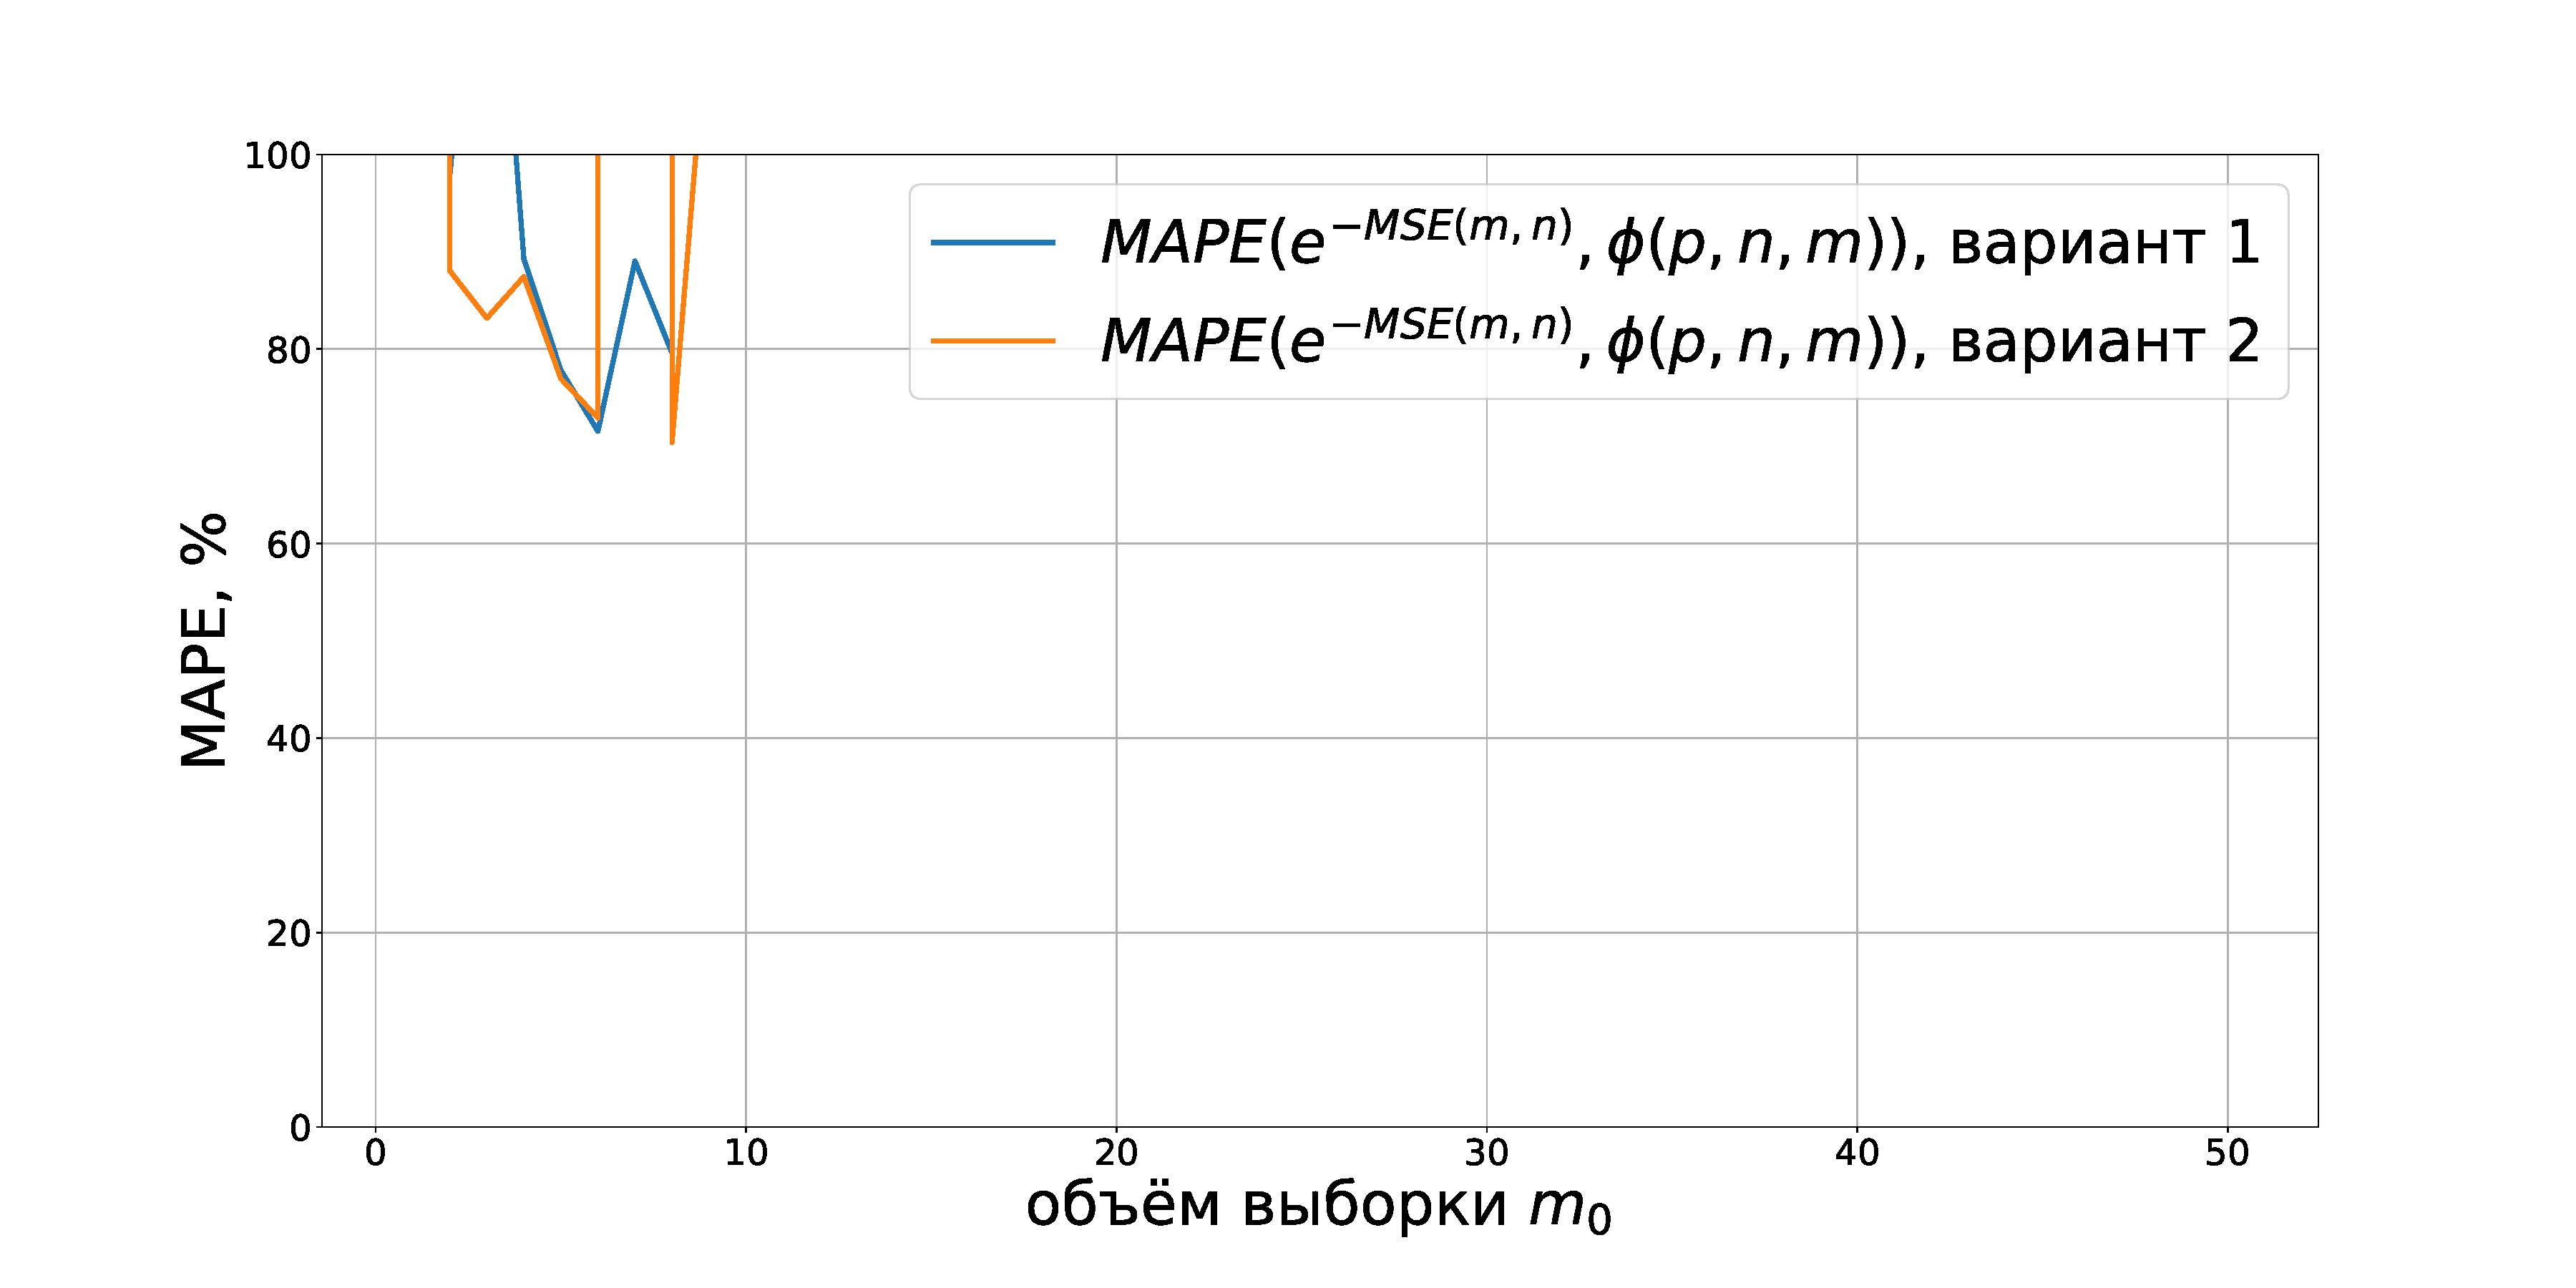
\includegraphics[width=0.55\textwidth]{../data/pics/adequate_redundant_sample_MAPE_comparison.pdf}}&
\subfloat{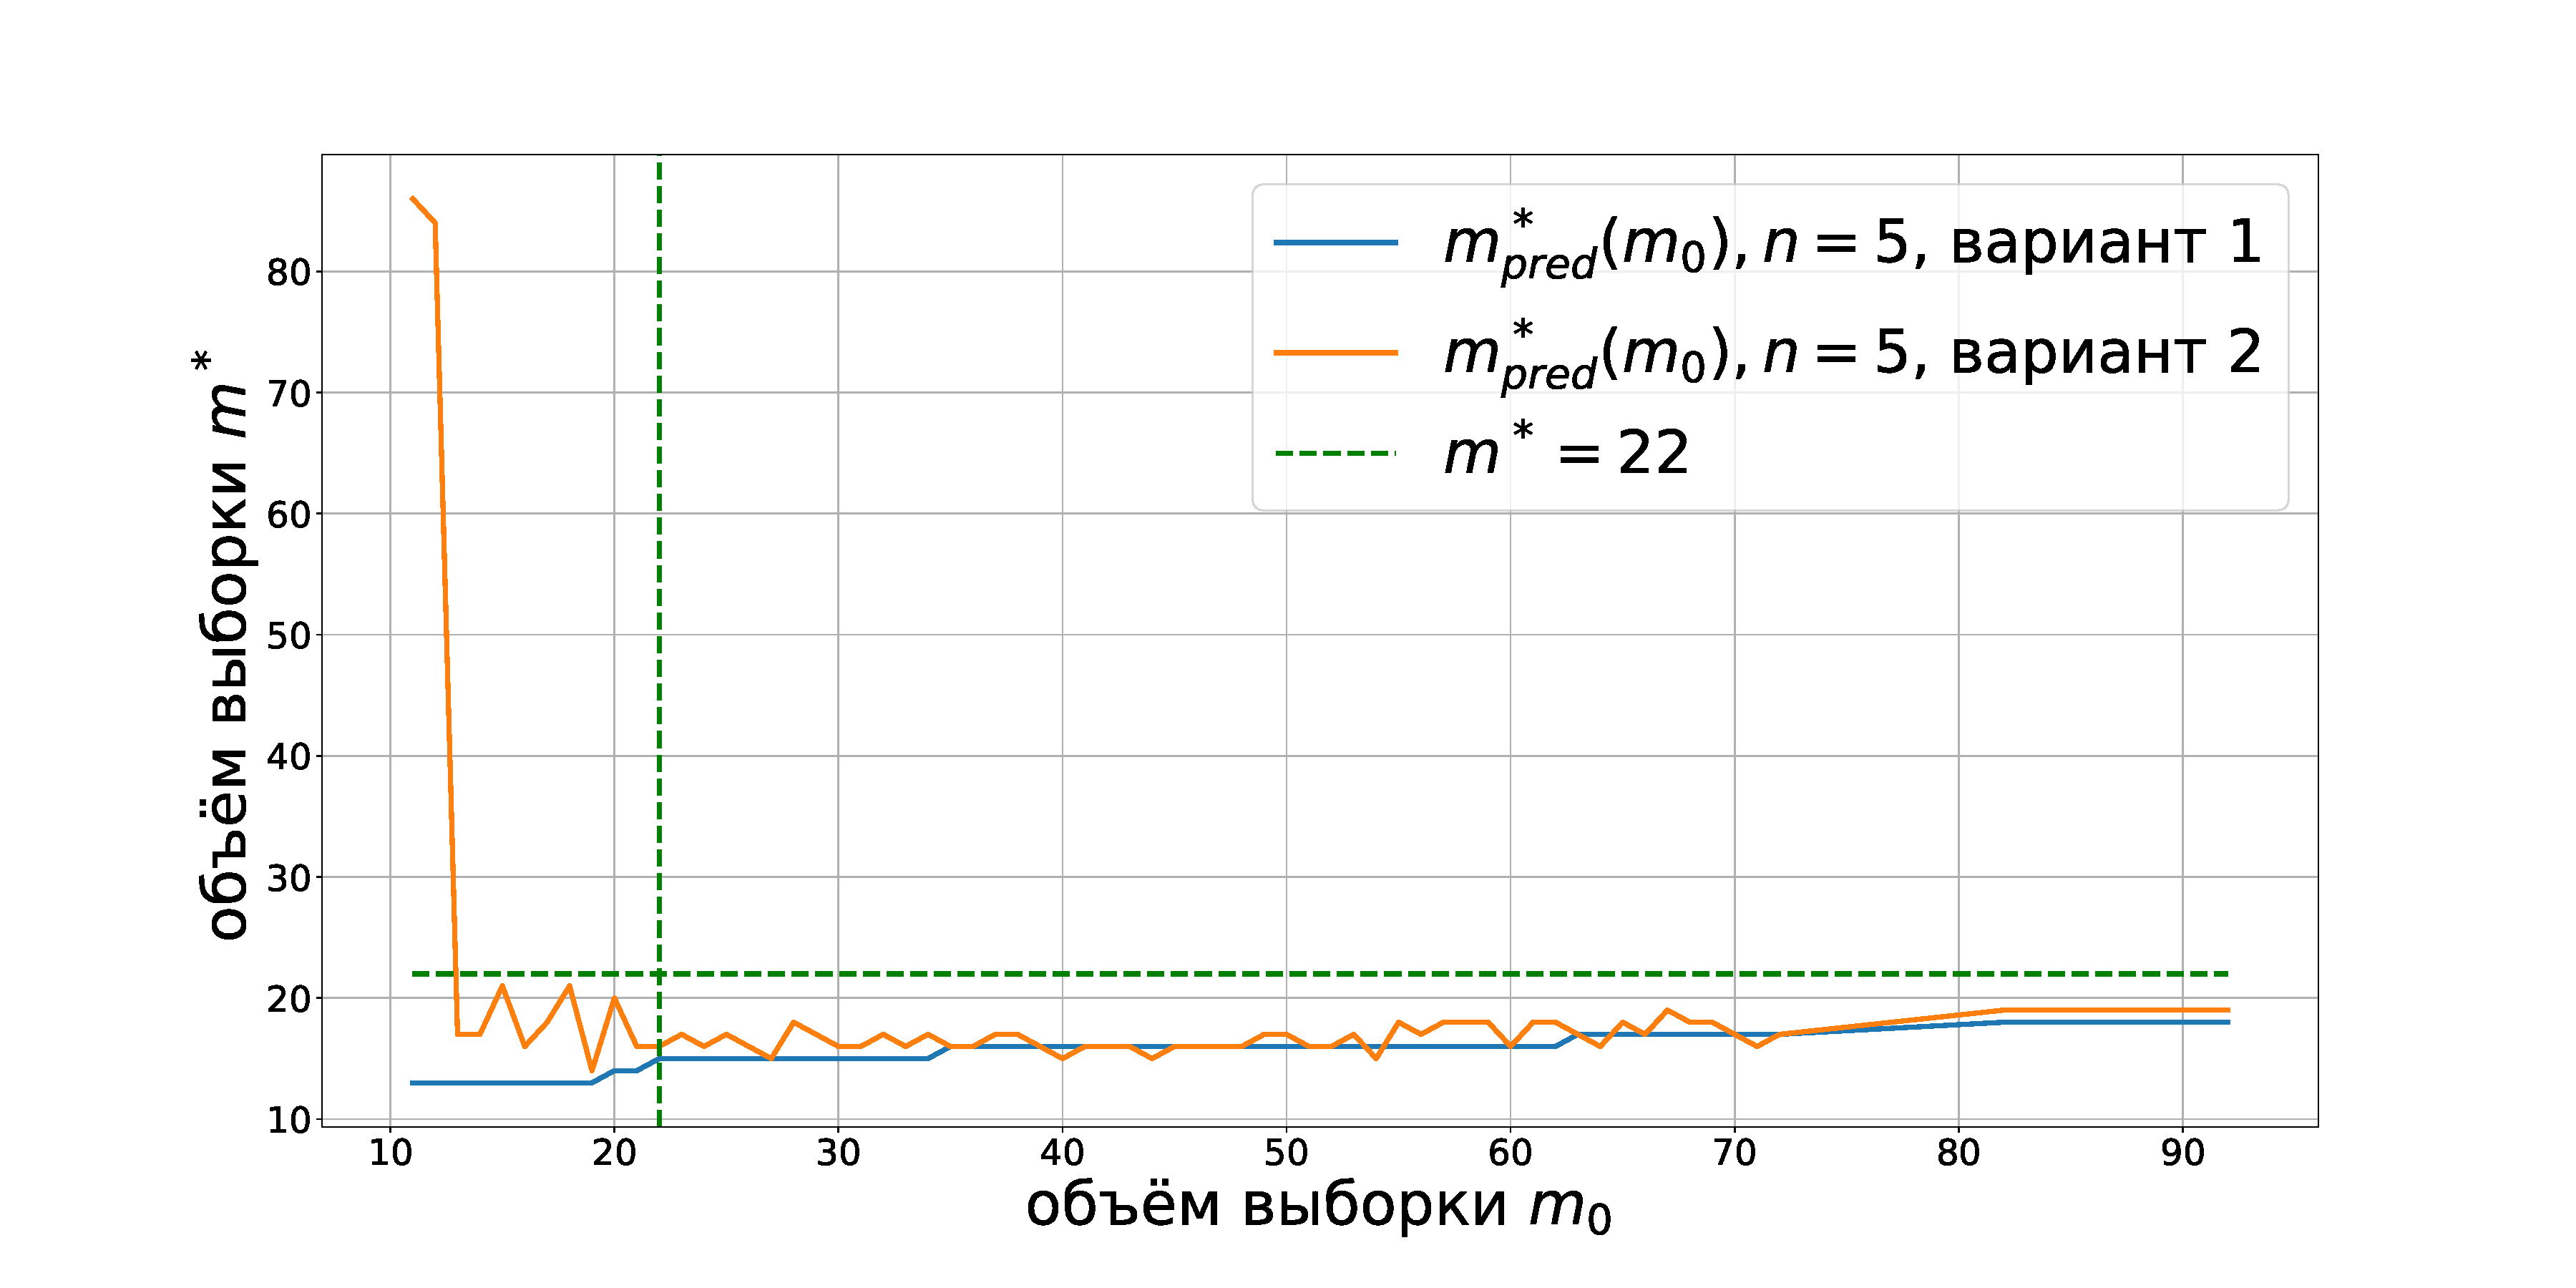
\includegraphics[width=0.55\textwidth]{../data/pics/adequate_redundant_sample_MAPE_m_comparison_n5.pdf}}\\
\end{tabular}

\caption{Качество предсказания $e^{-S(m, n)}$ и $m^*$ в зависимости от объема обучающей выборки $m_0$ для избыточной конфигурации выборки}
\label{fig2}
\end{figure}

\end{frame}

\begin{frame}{Выборки из UCI репозитория}

\begin{table}[h]
\begin{center}
\label{table3}
\begin{tabularx}{0.7\textwidth}{|c|>{\centering\arraybackslash}X|>{\centering\arraybackslash}X|>{\centering\arraybackslash}X|>{\centering\arraybackslash}X|}
\hline
	\centering Выборка & $m^*$ & $m$ & $n^*$ & $n$\\
	\hline
	Diabetes & 96 & 221 & 11 & 11\\
	\hline
	Boston & 102 & 253 & 14 & 14\\
	\hline
	Wine & 27 & 65 & 14 & 14\\
	\hline
	Nba & 38 & 200 & 20 & 20\\
\hline
\end{tabularx}
\end{center}
\end{table}

\end{frame}

\begin{frame}
\frametitle{Результаты эксперимента на выборках из UCI репозитория}

\begin{figure}[h!t]\center
\centering\begin{tabular}{@{}c@{ }c@{ }c@{}}
\textbf{Матожидание} & \textbf{Дисперсия}\\
\subfloat{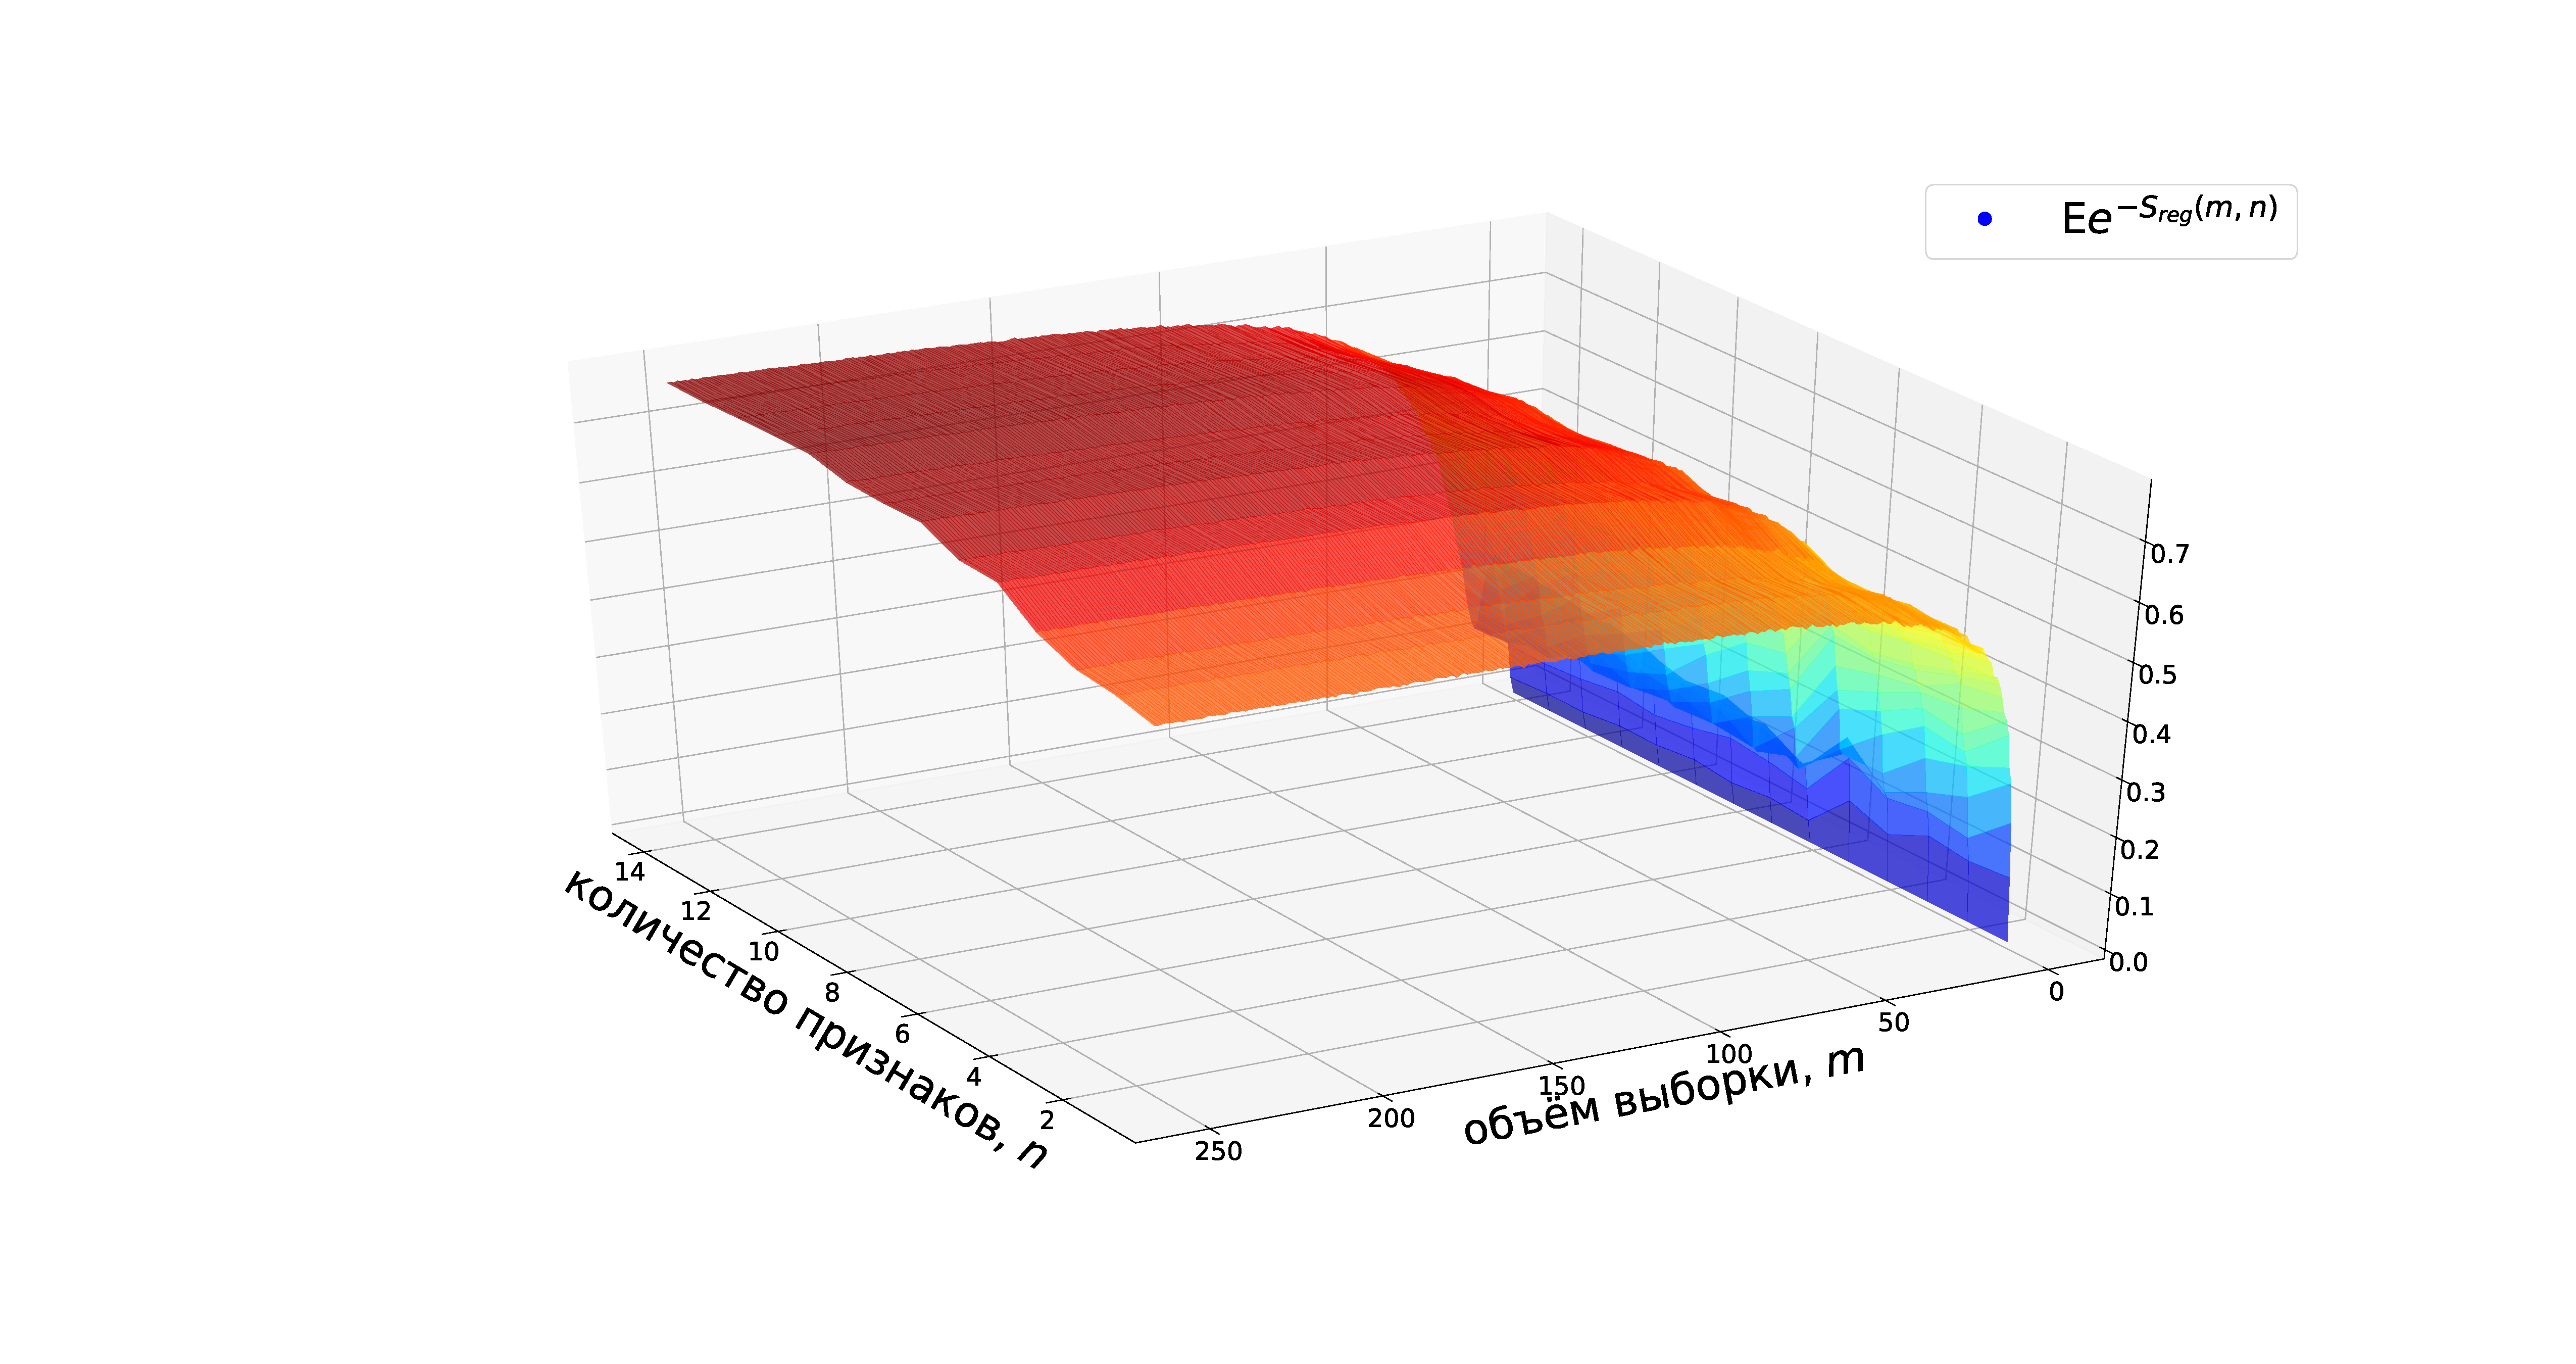
\includegraphics[width=0.5\textwidth]{../data/pics/boston_sample_llh.pdf}}&
\subfloat{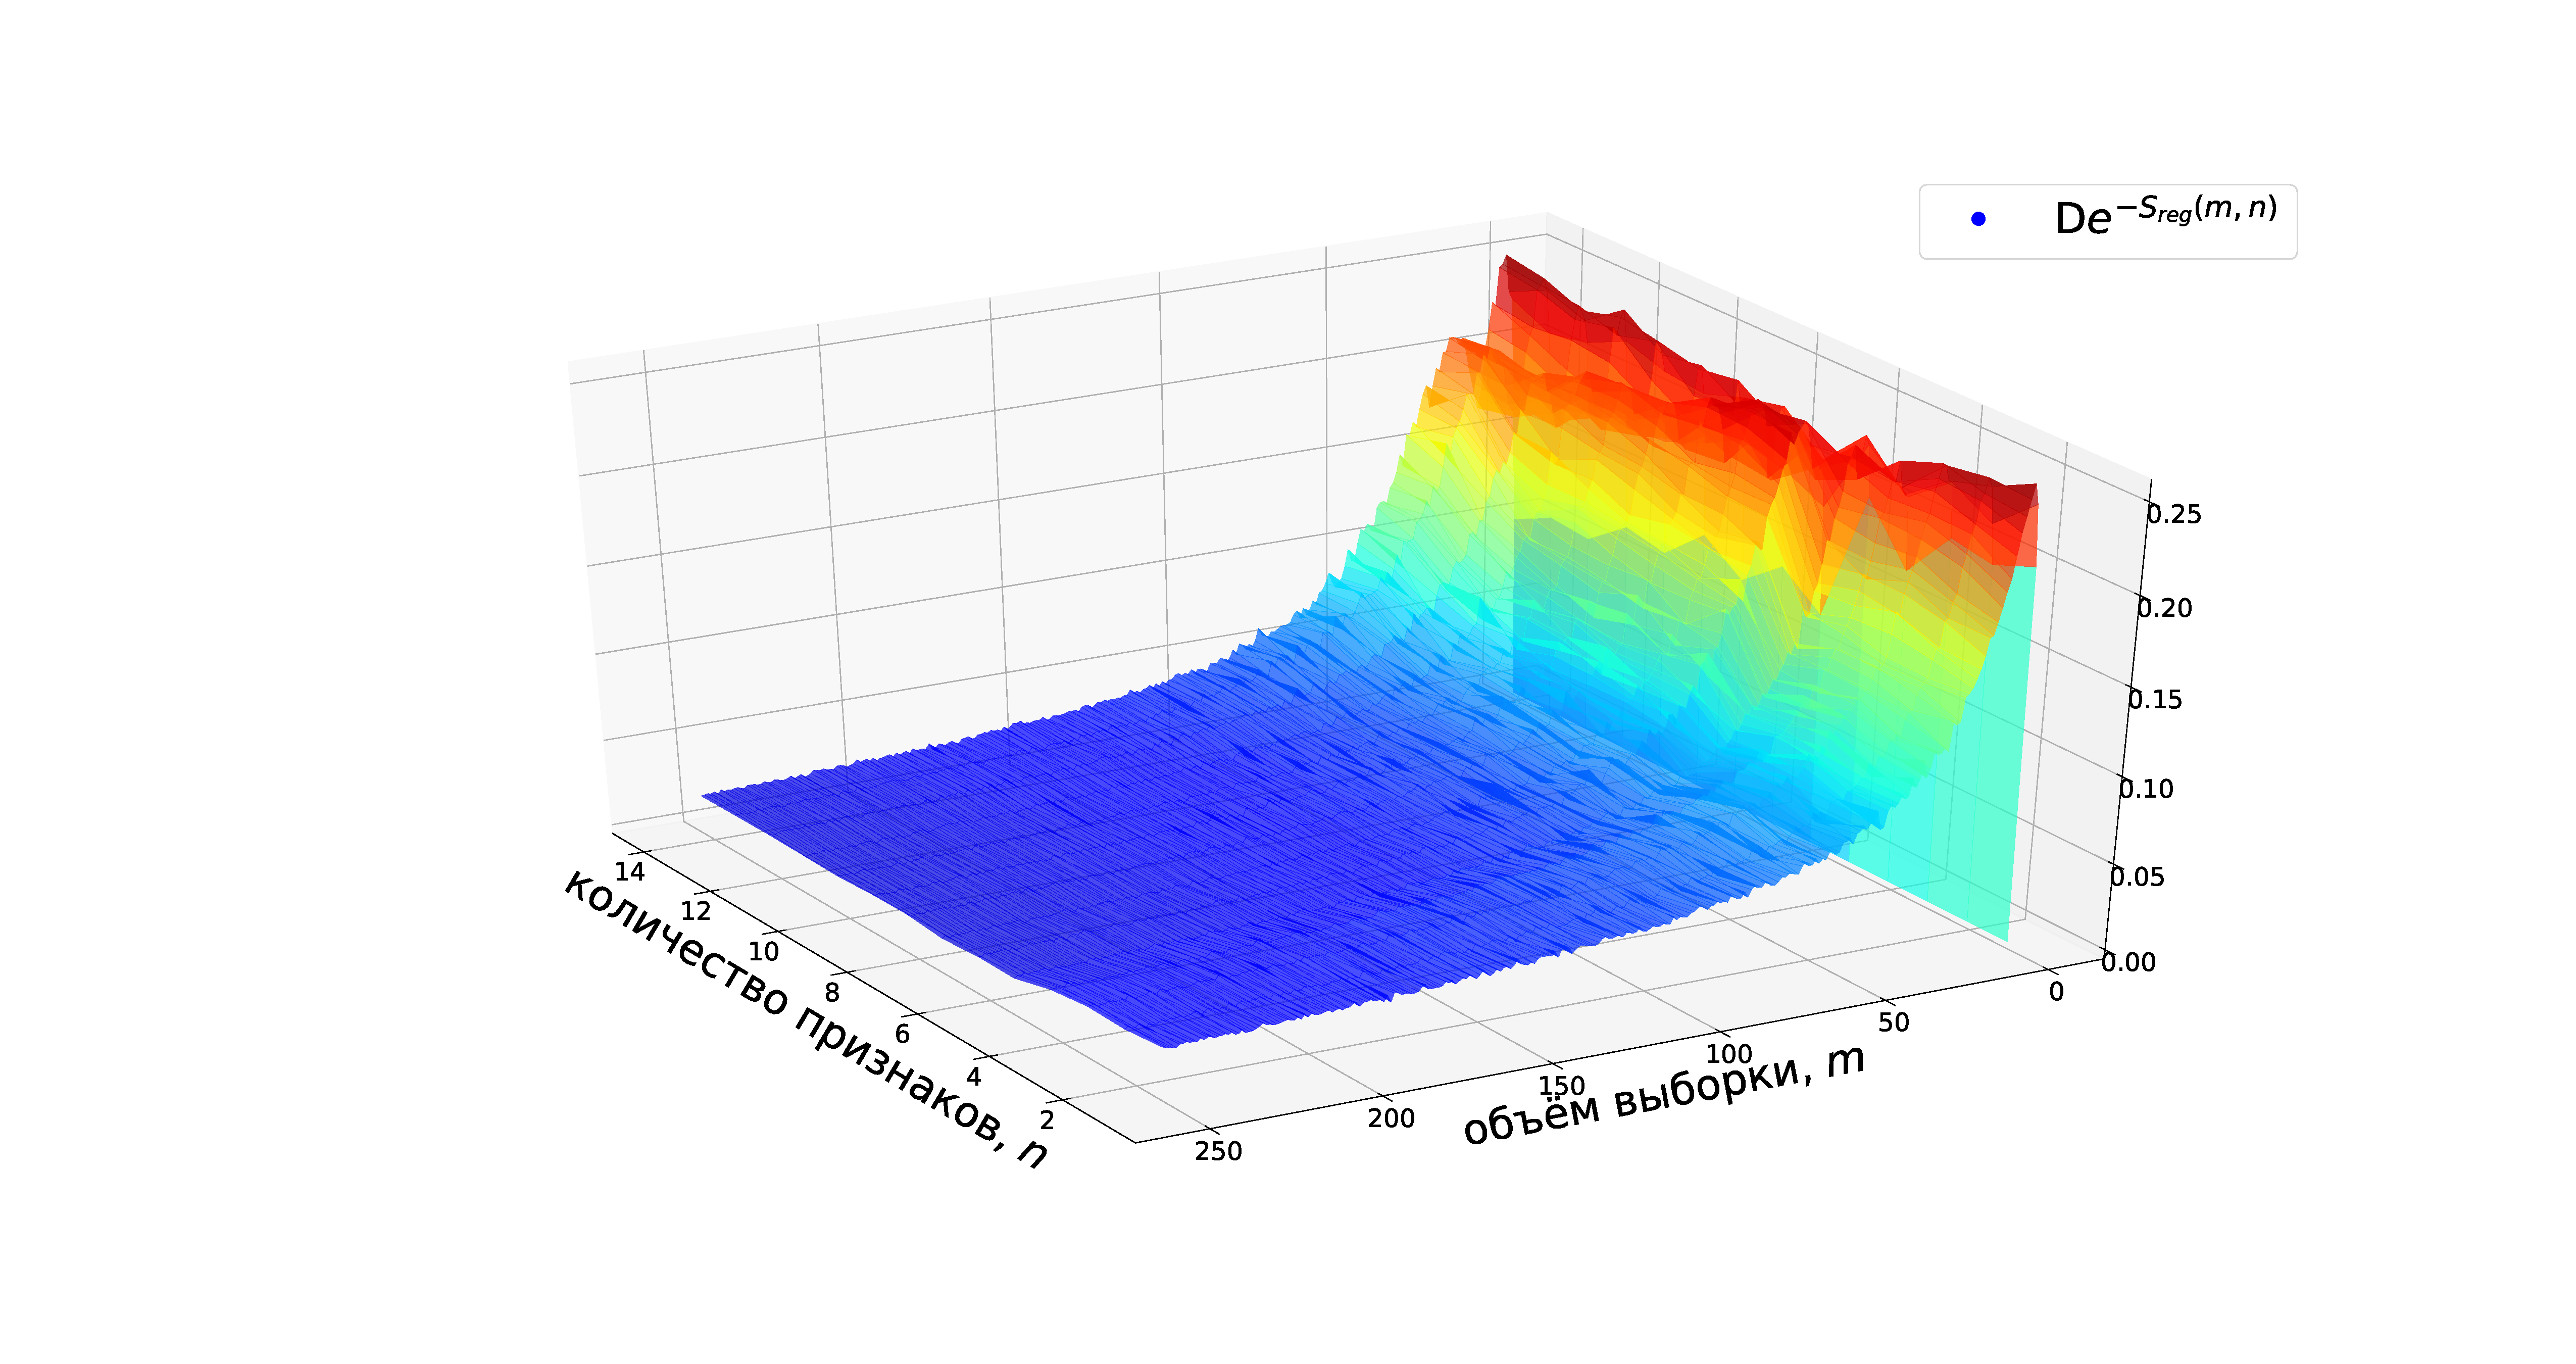
\includegraphics[width=0.5\textwidth]{../data/pics/boston_sample_llh_std.pdf}}\\
\end{tabular}

\caption{Зависимость значения функции $e^{-S(m, n)}$ от объема выборки $m$ и количества параметров $n$ для выборки Boston}
\label{fig3}
\end{figure}

\end{frame}

\begin{frame}
\frametitle{Результаты эксперимента на выборках из UCI репозитория}

\begin{figure}[h!t]\center
\centering\begin{tabular}{@{}c@{ }c@{ }c@{}}
\textbf{Аппроксимация $e^{-S(m, n)}$} & \textbf{Предсказание $m^*$}\\
\subfloat{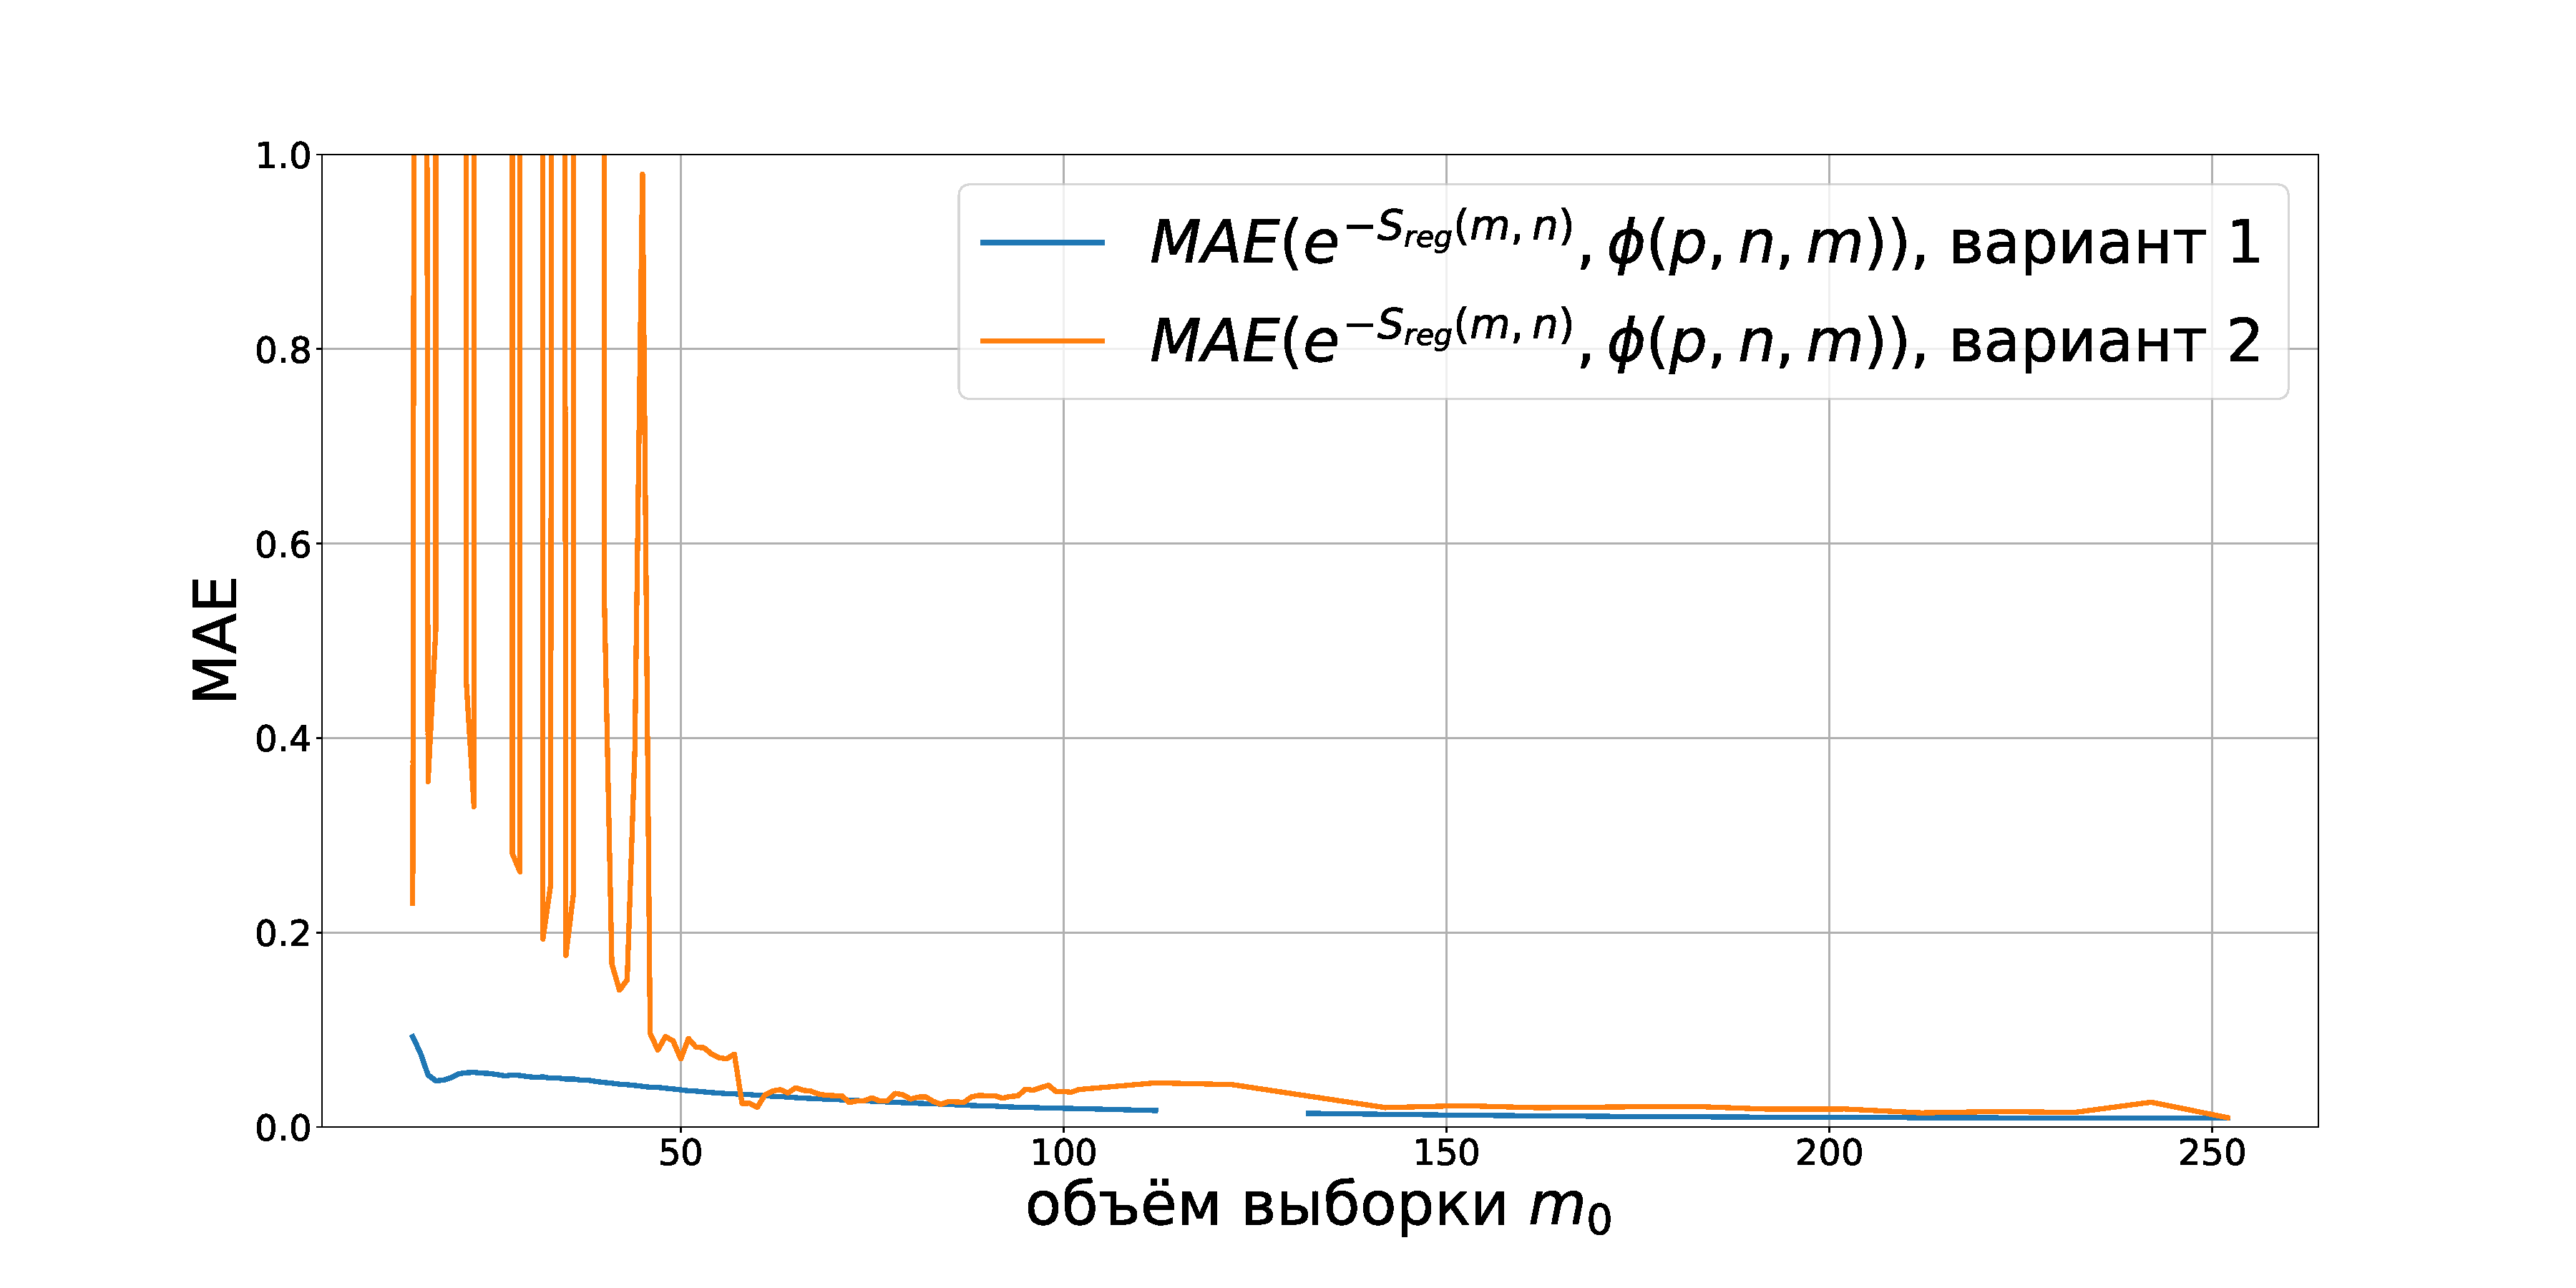
\includegraphics[width=0.5\textwidth]{../data/pics/boston_sample_MAPE_comparison.pdf}}&
\subfloat{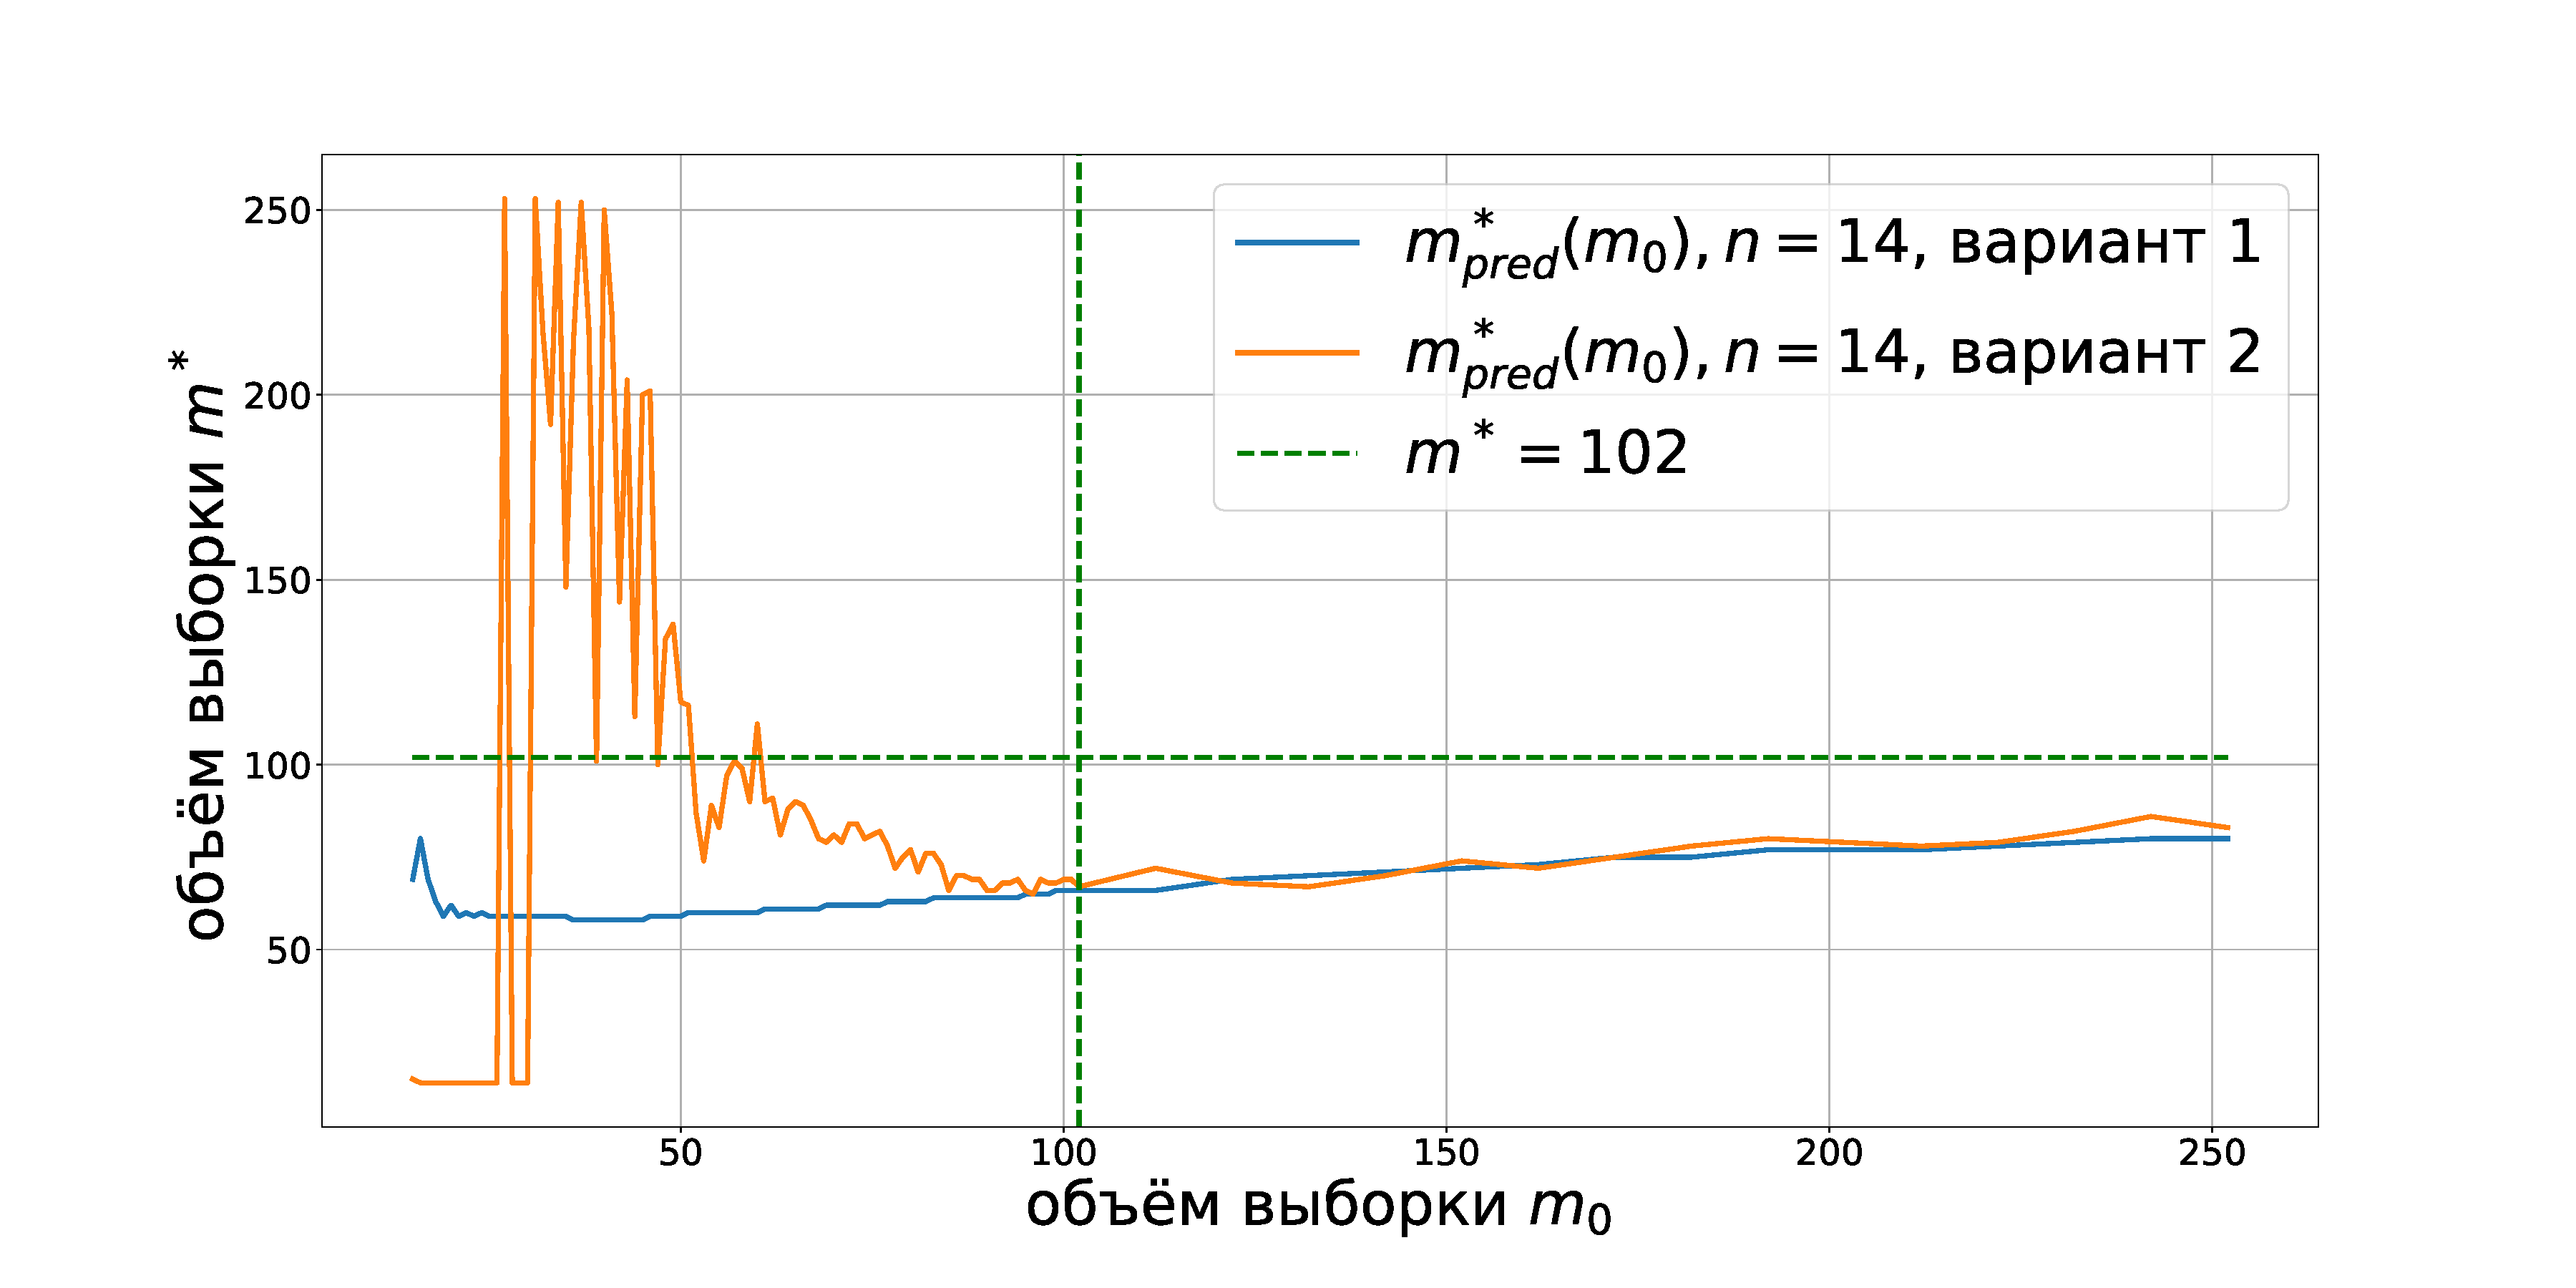
\includegraphics[width=0.5\textwidth]{../data/pics/boston_sample_MAPE_m_comparison_n14.pdf}}\\
\end{tabular}

\caption{Качество предсказания $e^{-S(m, n)}$ и $m^*$ в зависимости от объема обучающей выборки $m_0$ для выборки Boston}
\label{fig103}
\end{figure}

\end{frame}

\begin{frame}
\frametitle{Результаты эксперимента на выборках из UCI репозитория}

\begin{figure}[h!t]\center
\centering\begin{tabular}{@{}c@{ }c@{ }c@{}}
\textbf{Матожидание} & \textbf{Дисперсия}\\
\subfloat{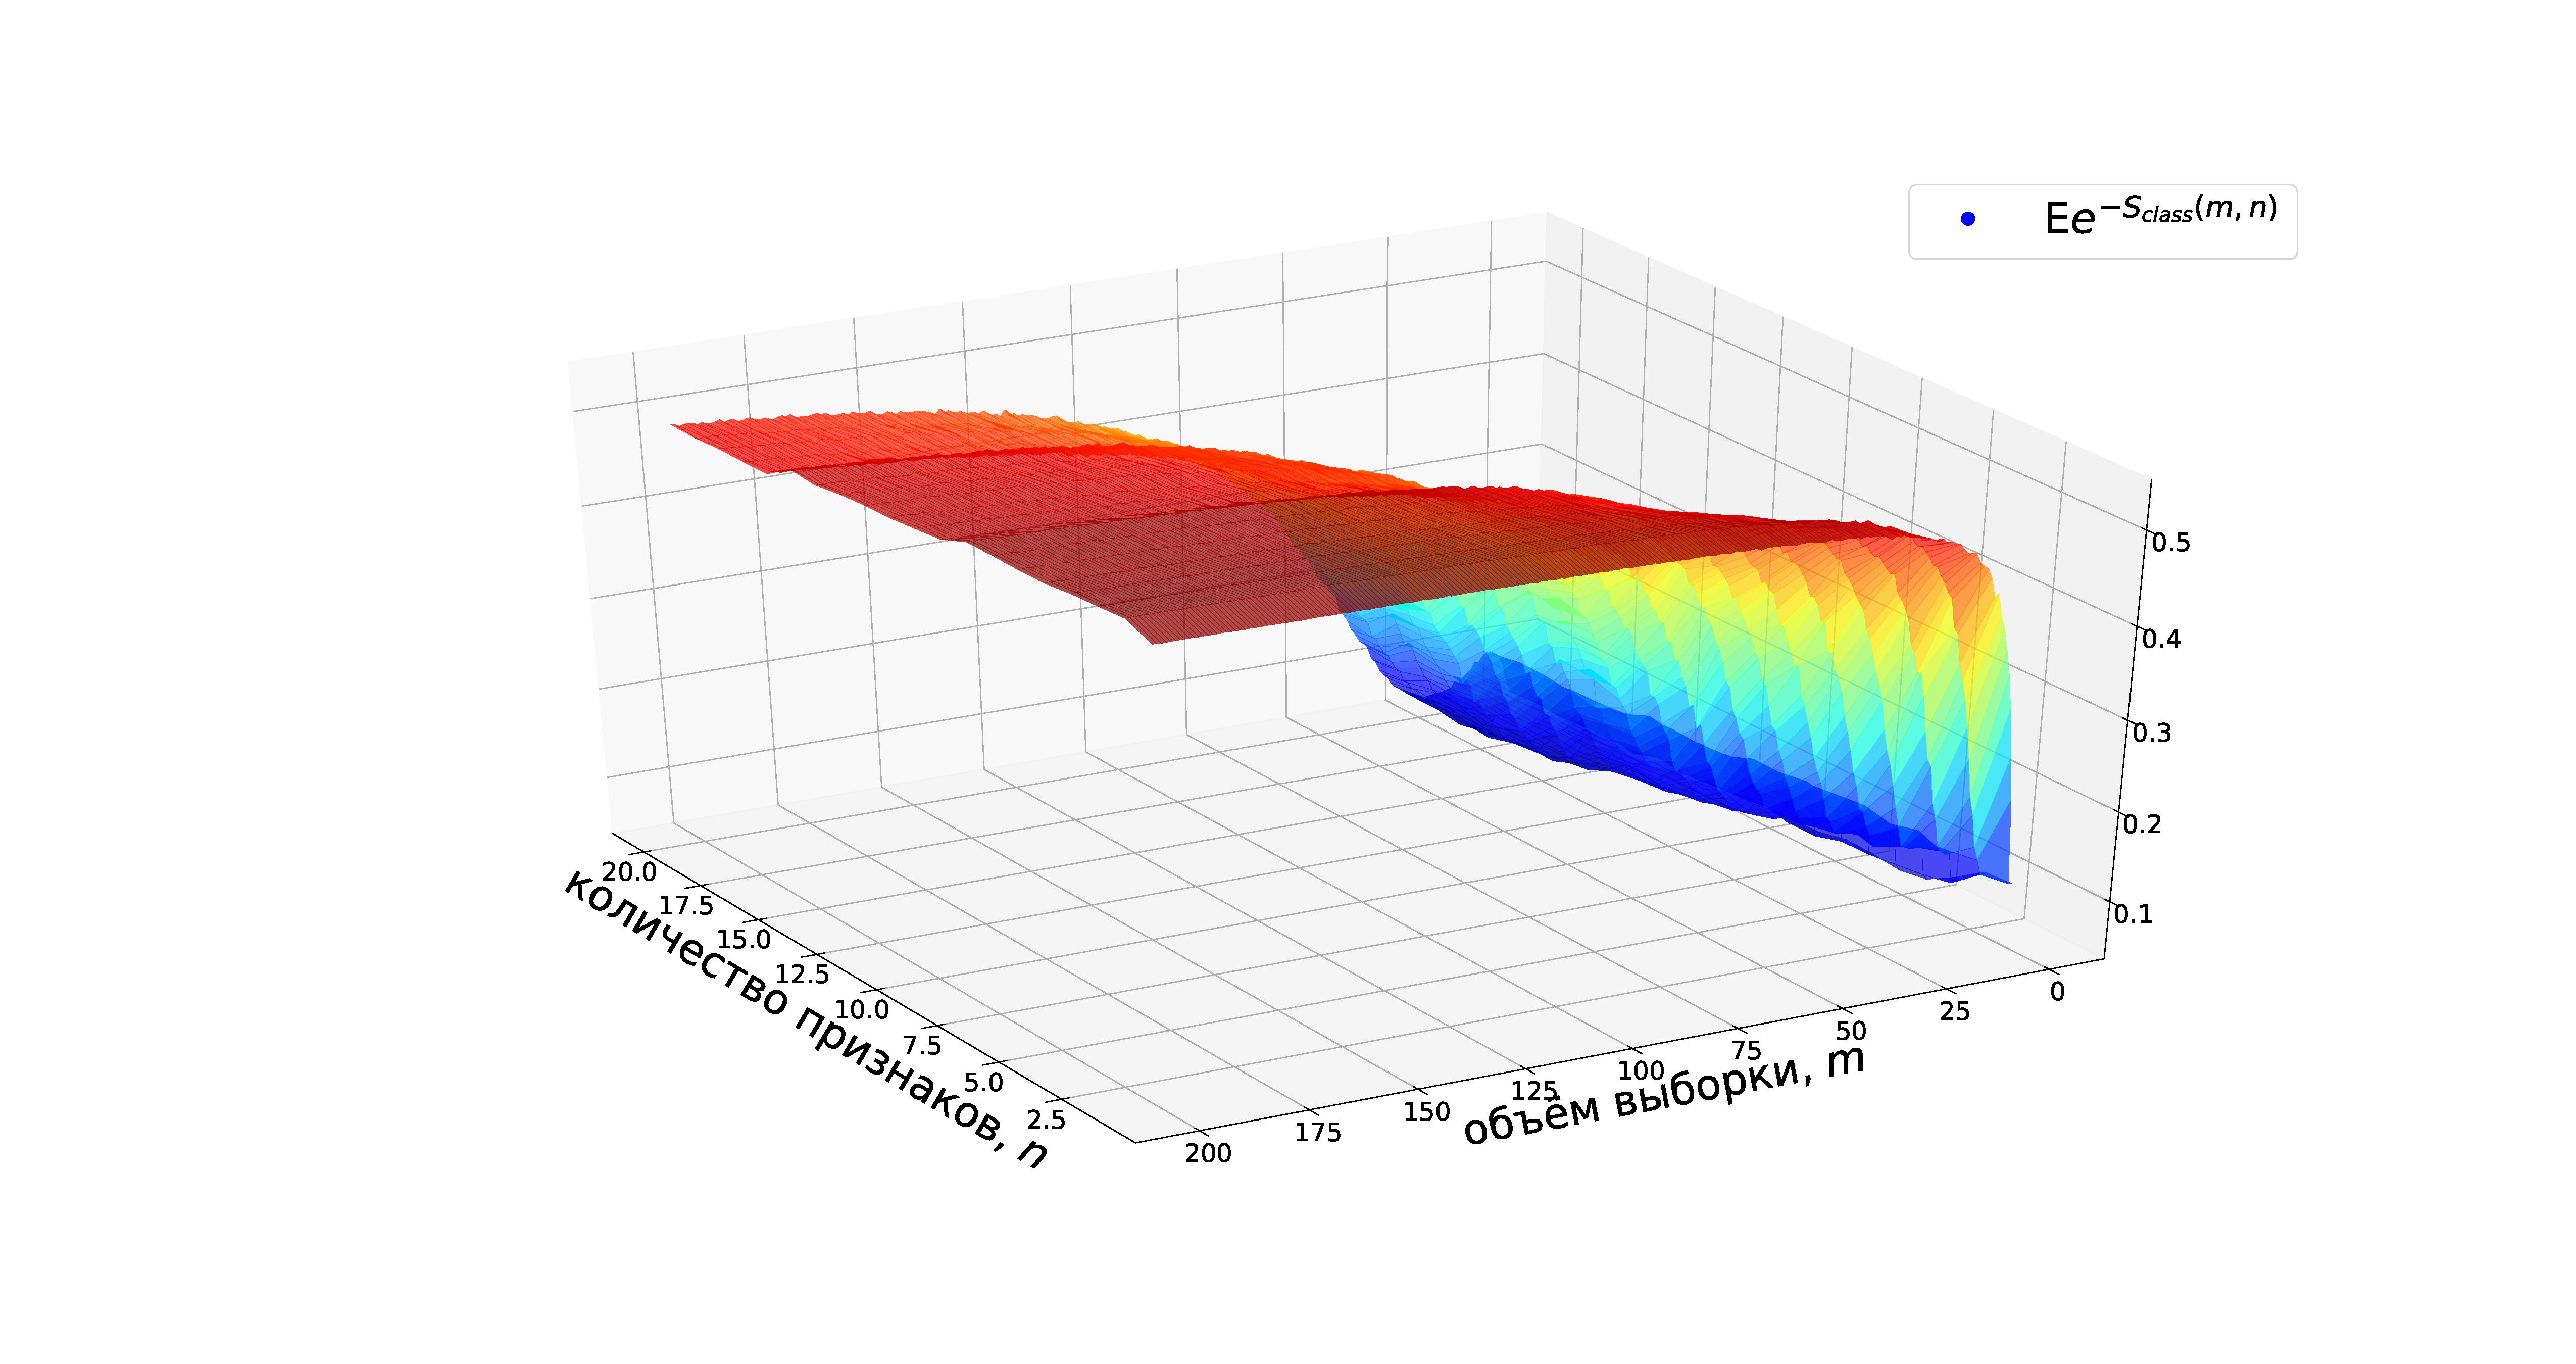
\includegraphics[width=0.5\textwidth]{../data/pics/nba_sample_llh.pdf}}&
\subfloat{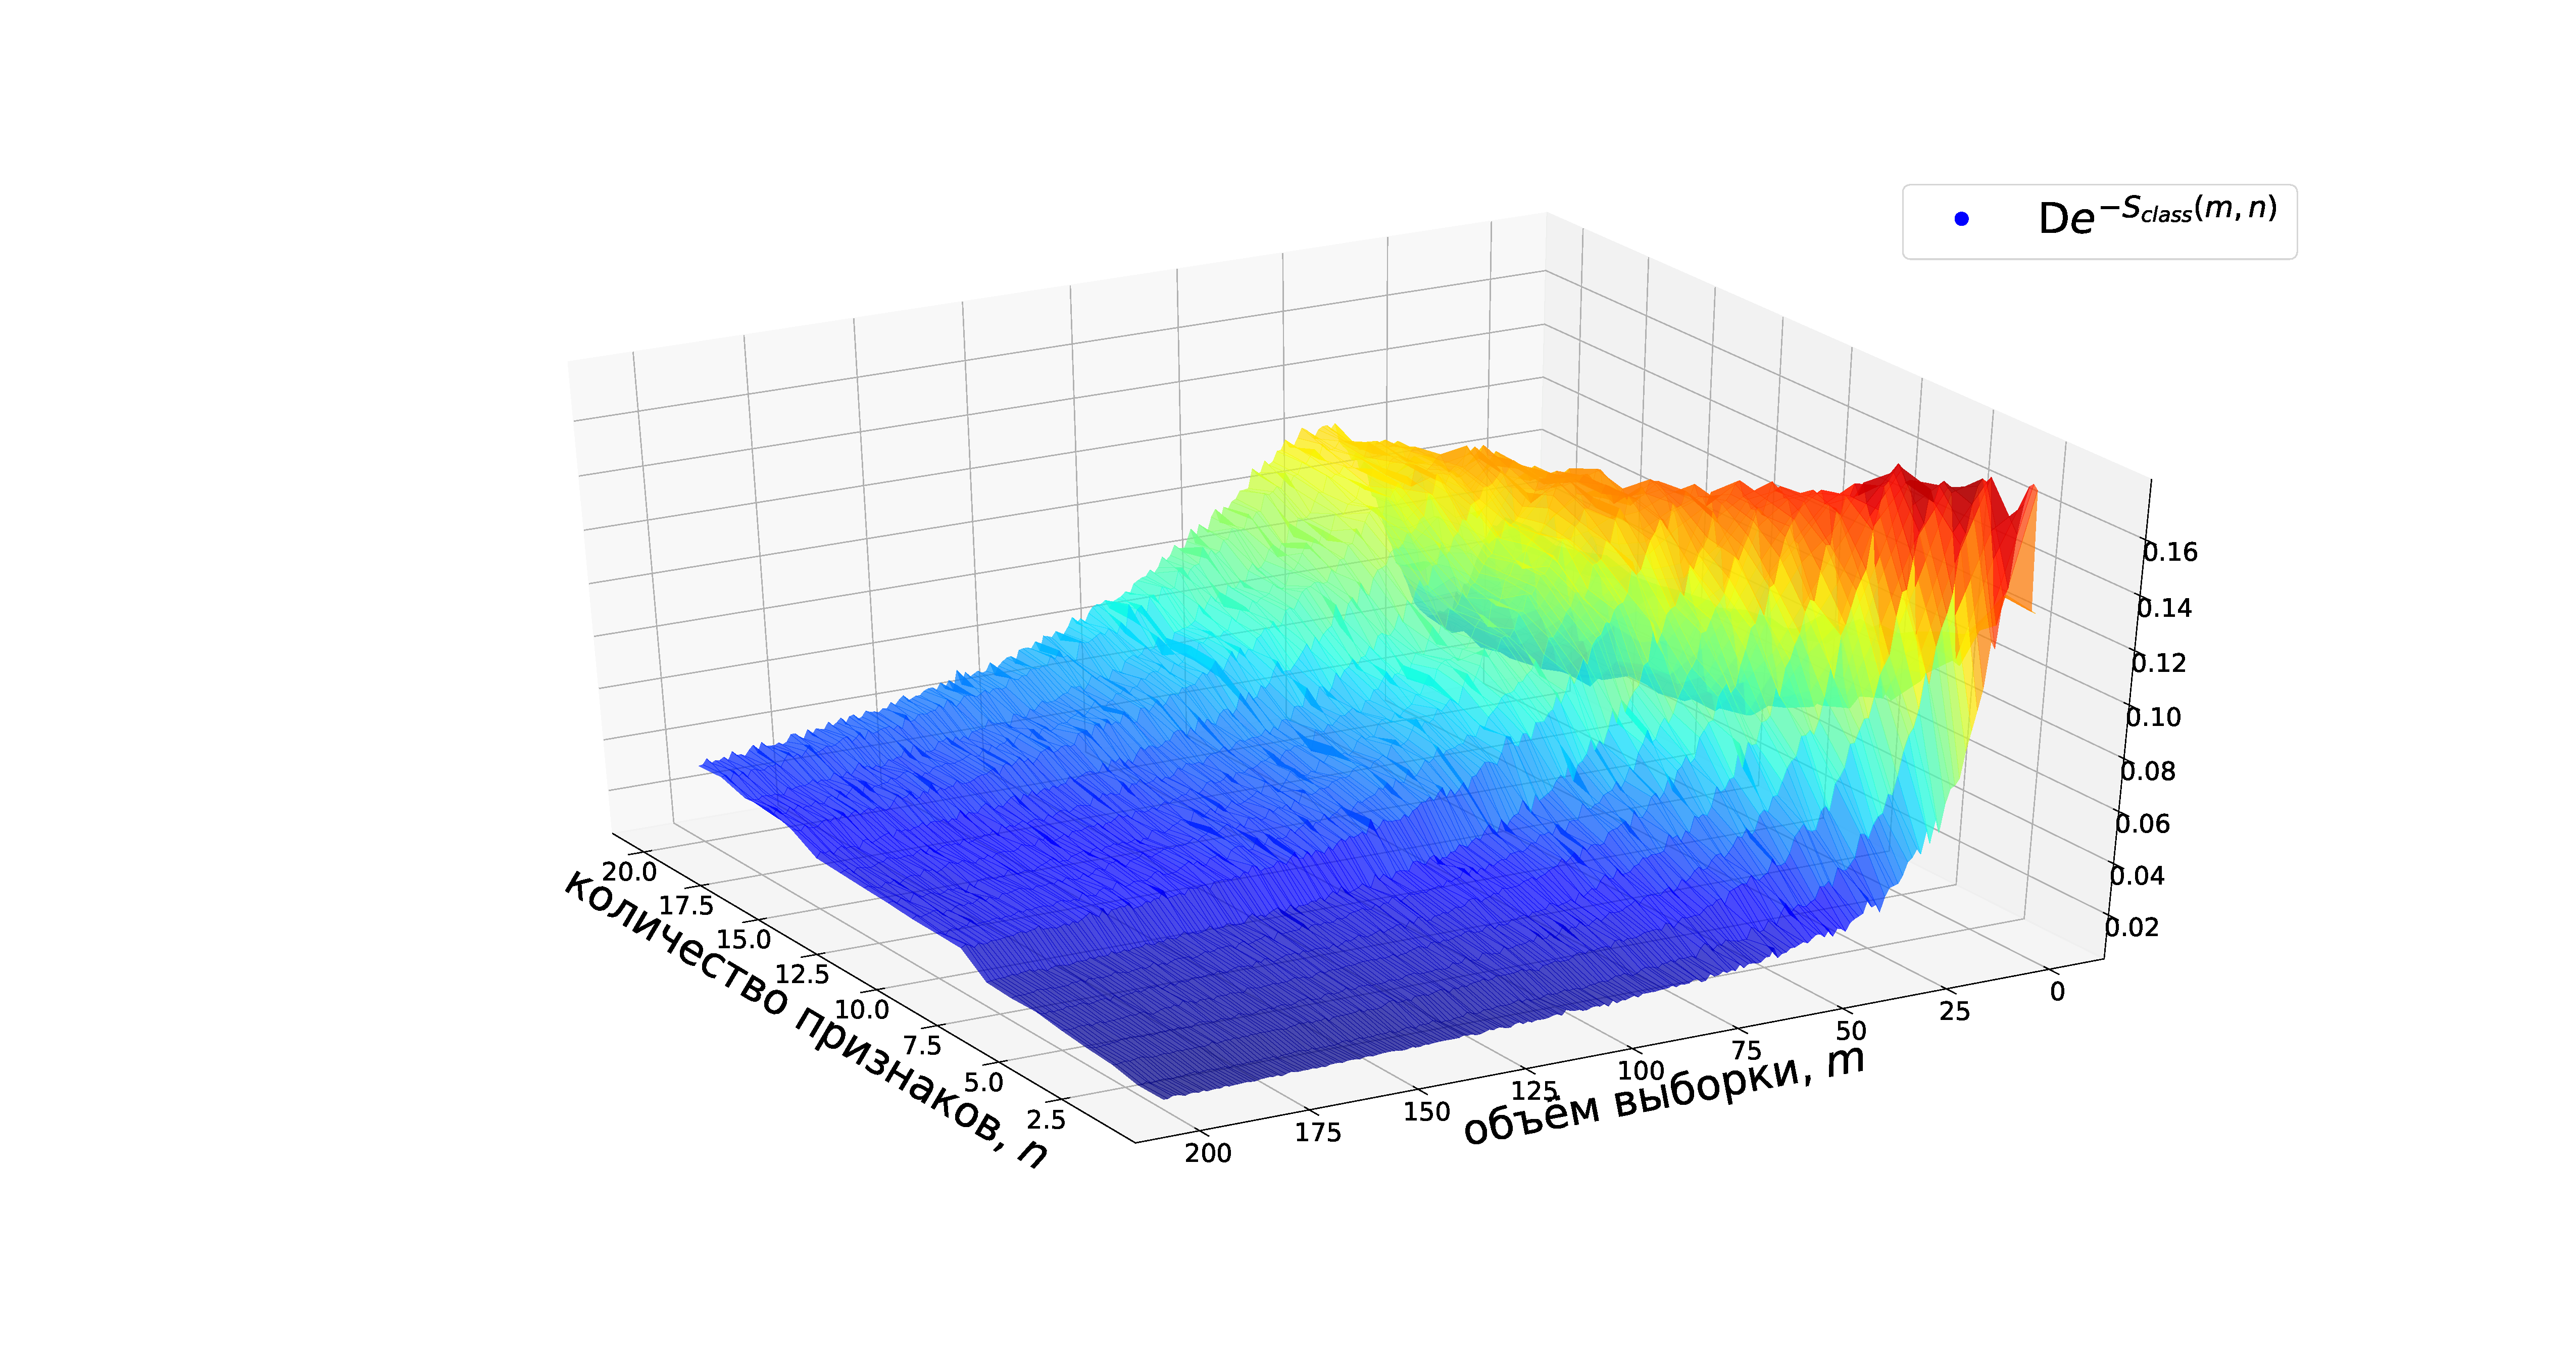
\includegraphics[width=0.5\textwidth]{../data/pics/nba_sample_llh_std.pdf}}\\
\end{tabular}

\caption{Зависимость значения функции $e^{-S(m, n)}$ от объема выборки $m$ и количества параметров $n$ для выборки Nba}
\label{fig3}
\end{figure}

\end{frame}

\begin{frame}
\frametitle{Результаты эксперимента на выборках из UCI репозитория}

\begin{figure}[h!t]\center
\centering\begin{tabular}{@{}c@{ }c@{ }c@{}}
\textbf{Аппроксимация $e^{-S(m, n)}$} & \textbf{Предсказание $m^*$}\\
\subfloat{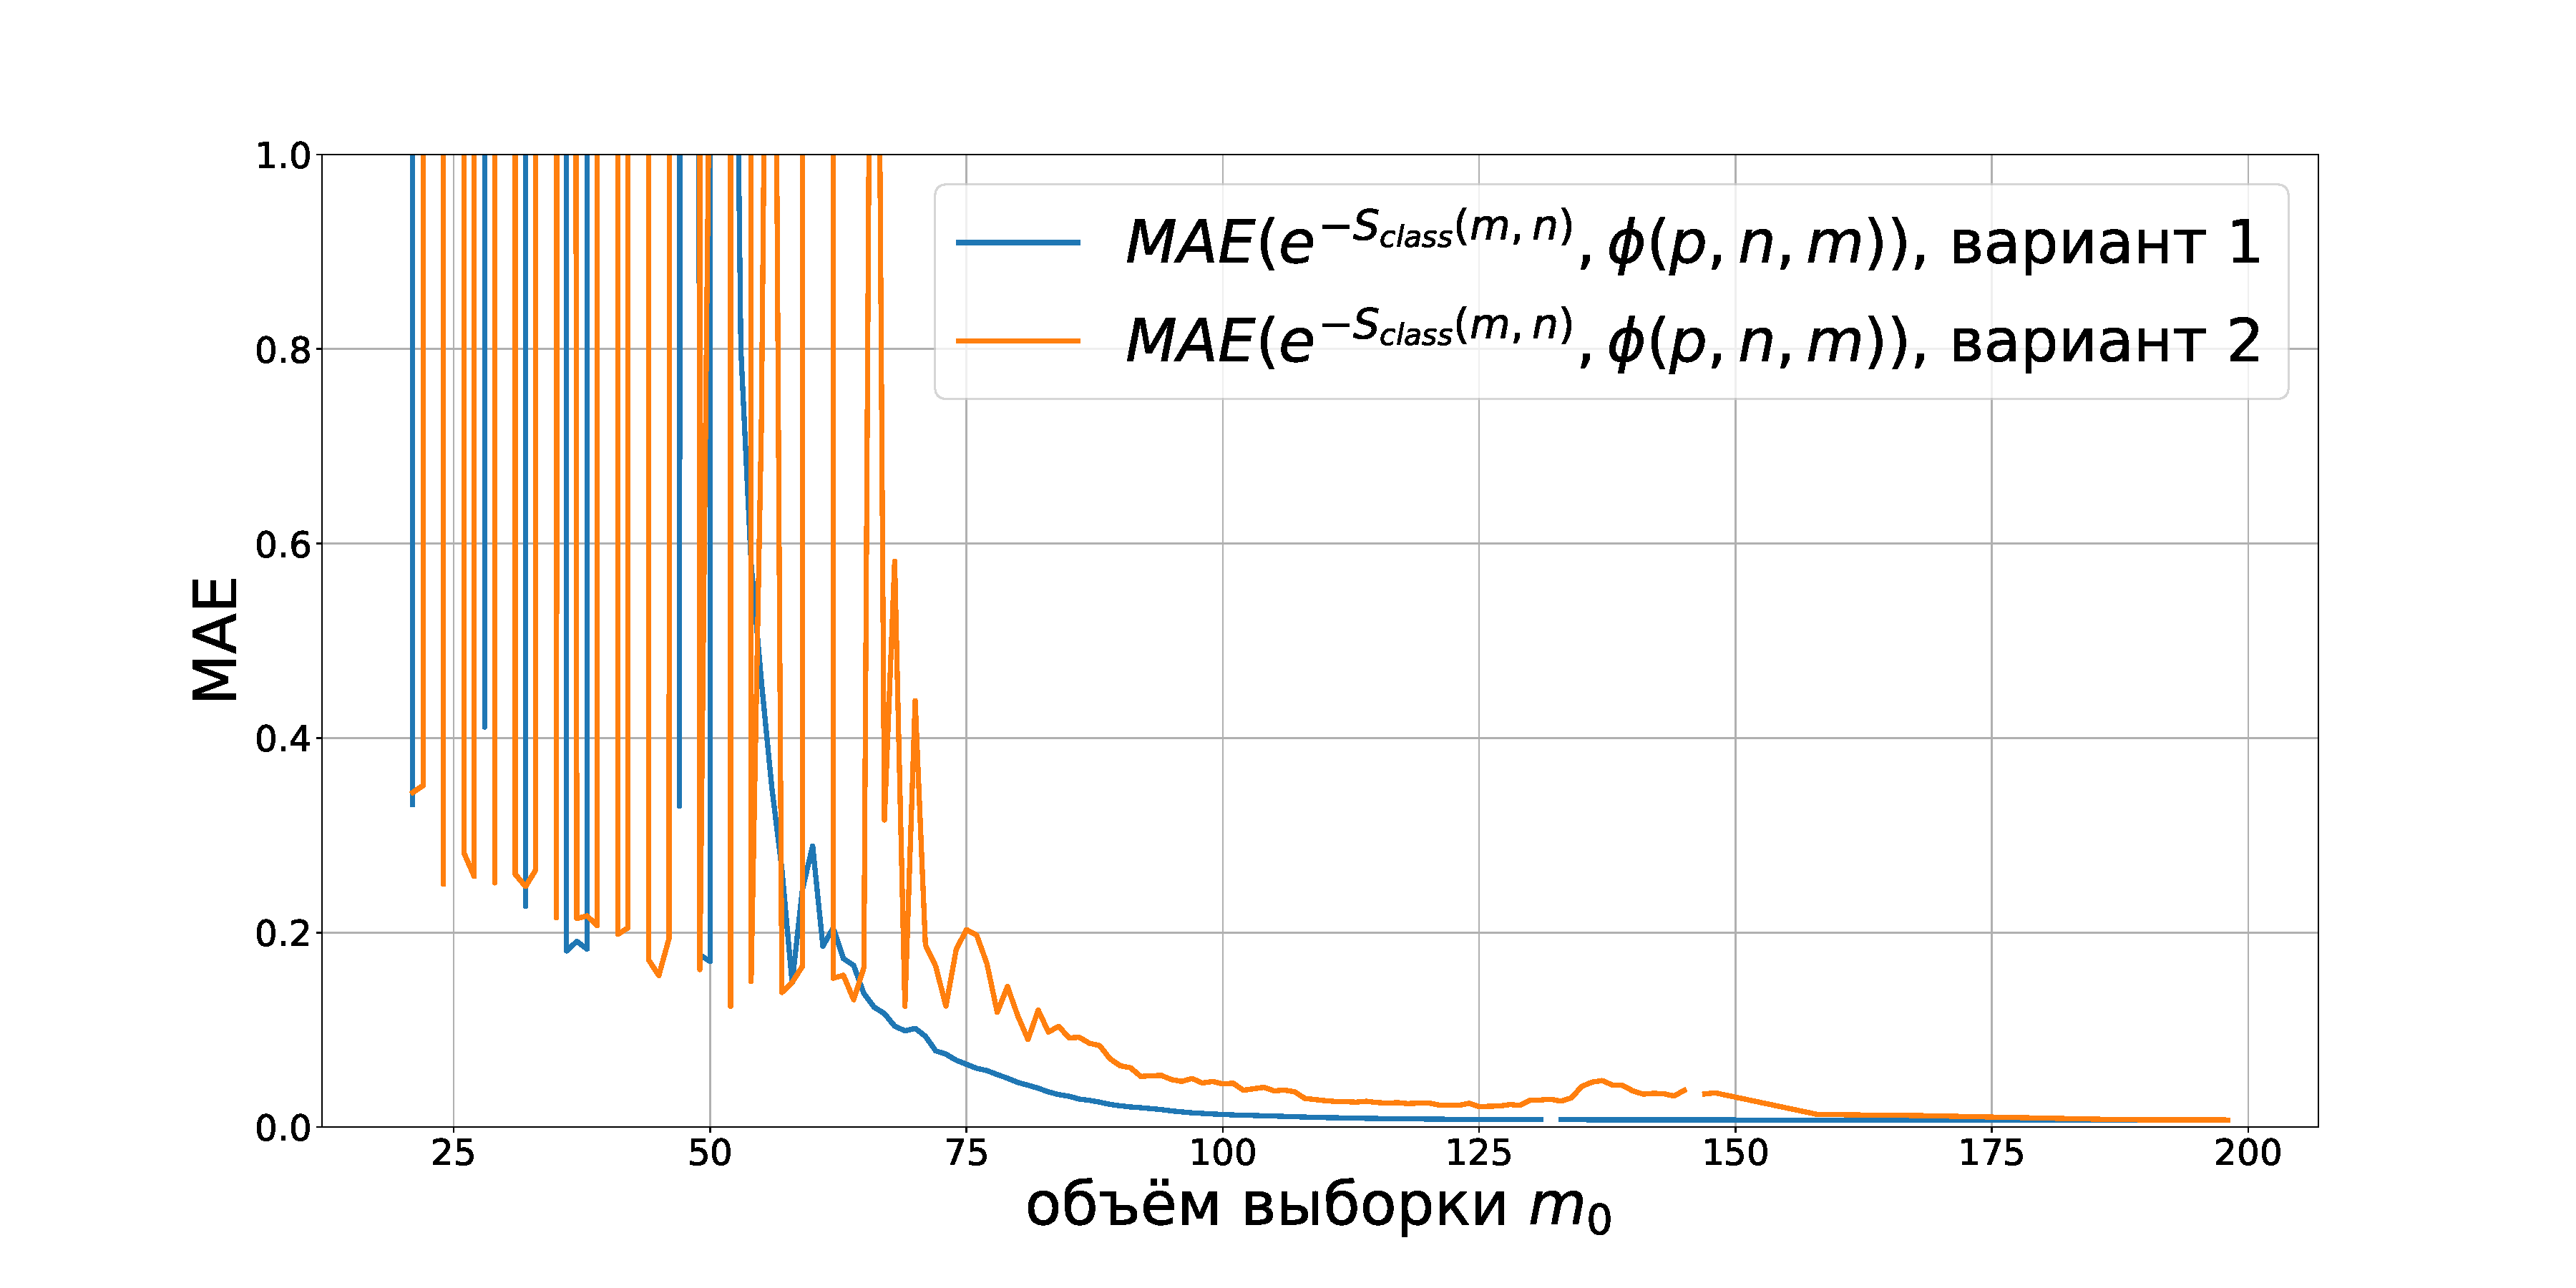
\includegraphics[width=0.5\textwidth]{../data/pics/nba_sample_MAPE_comparison.pdf}}&
\subfloat{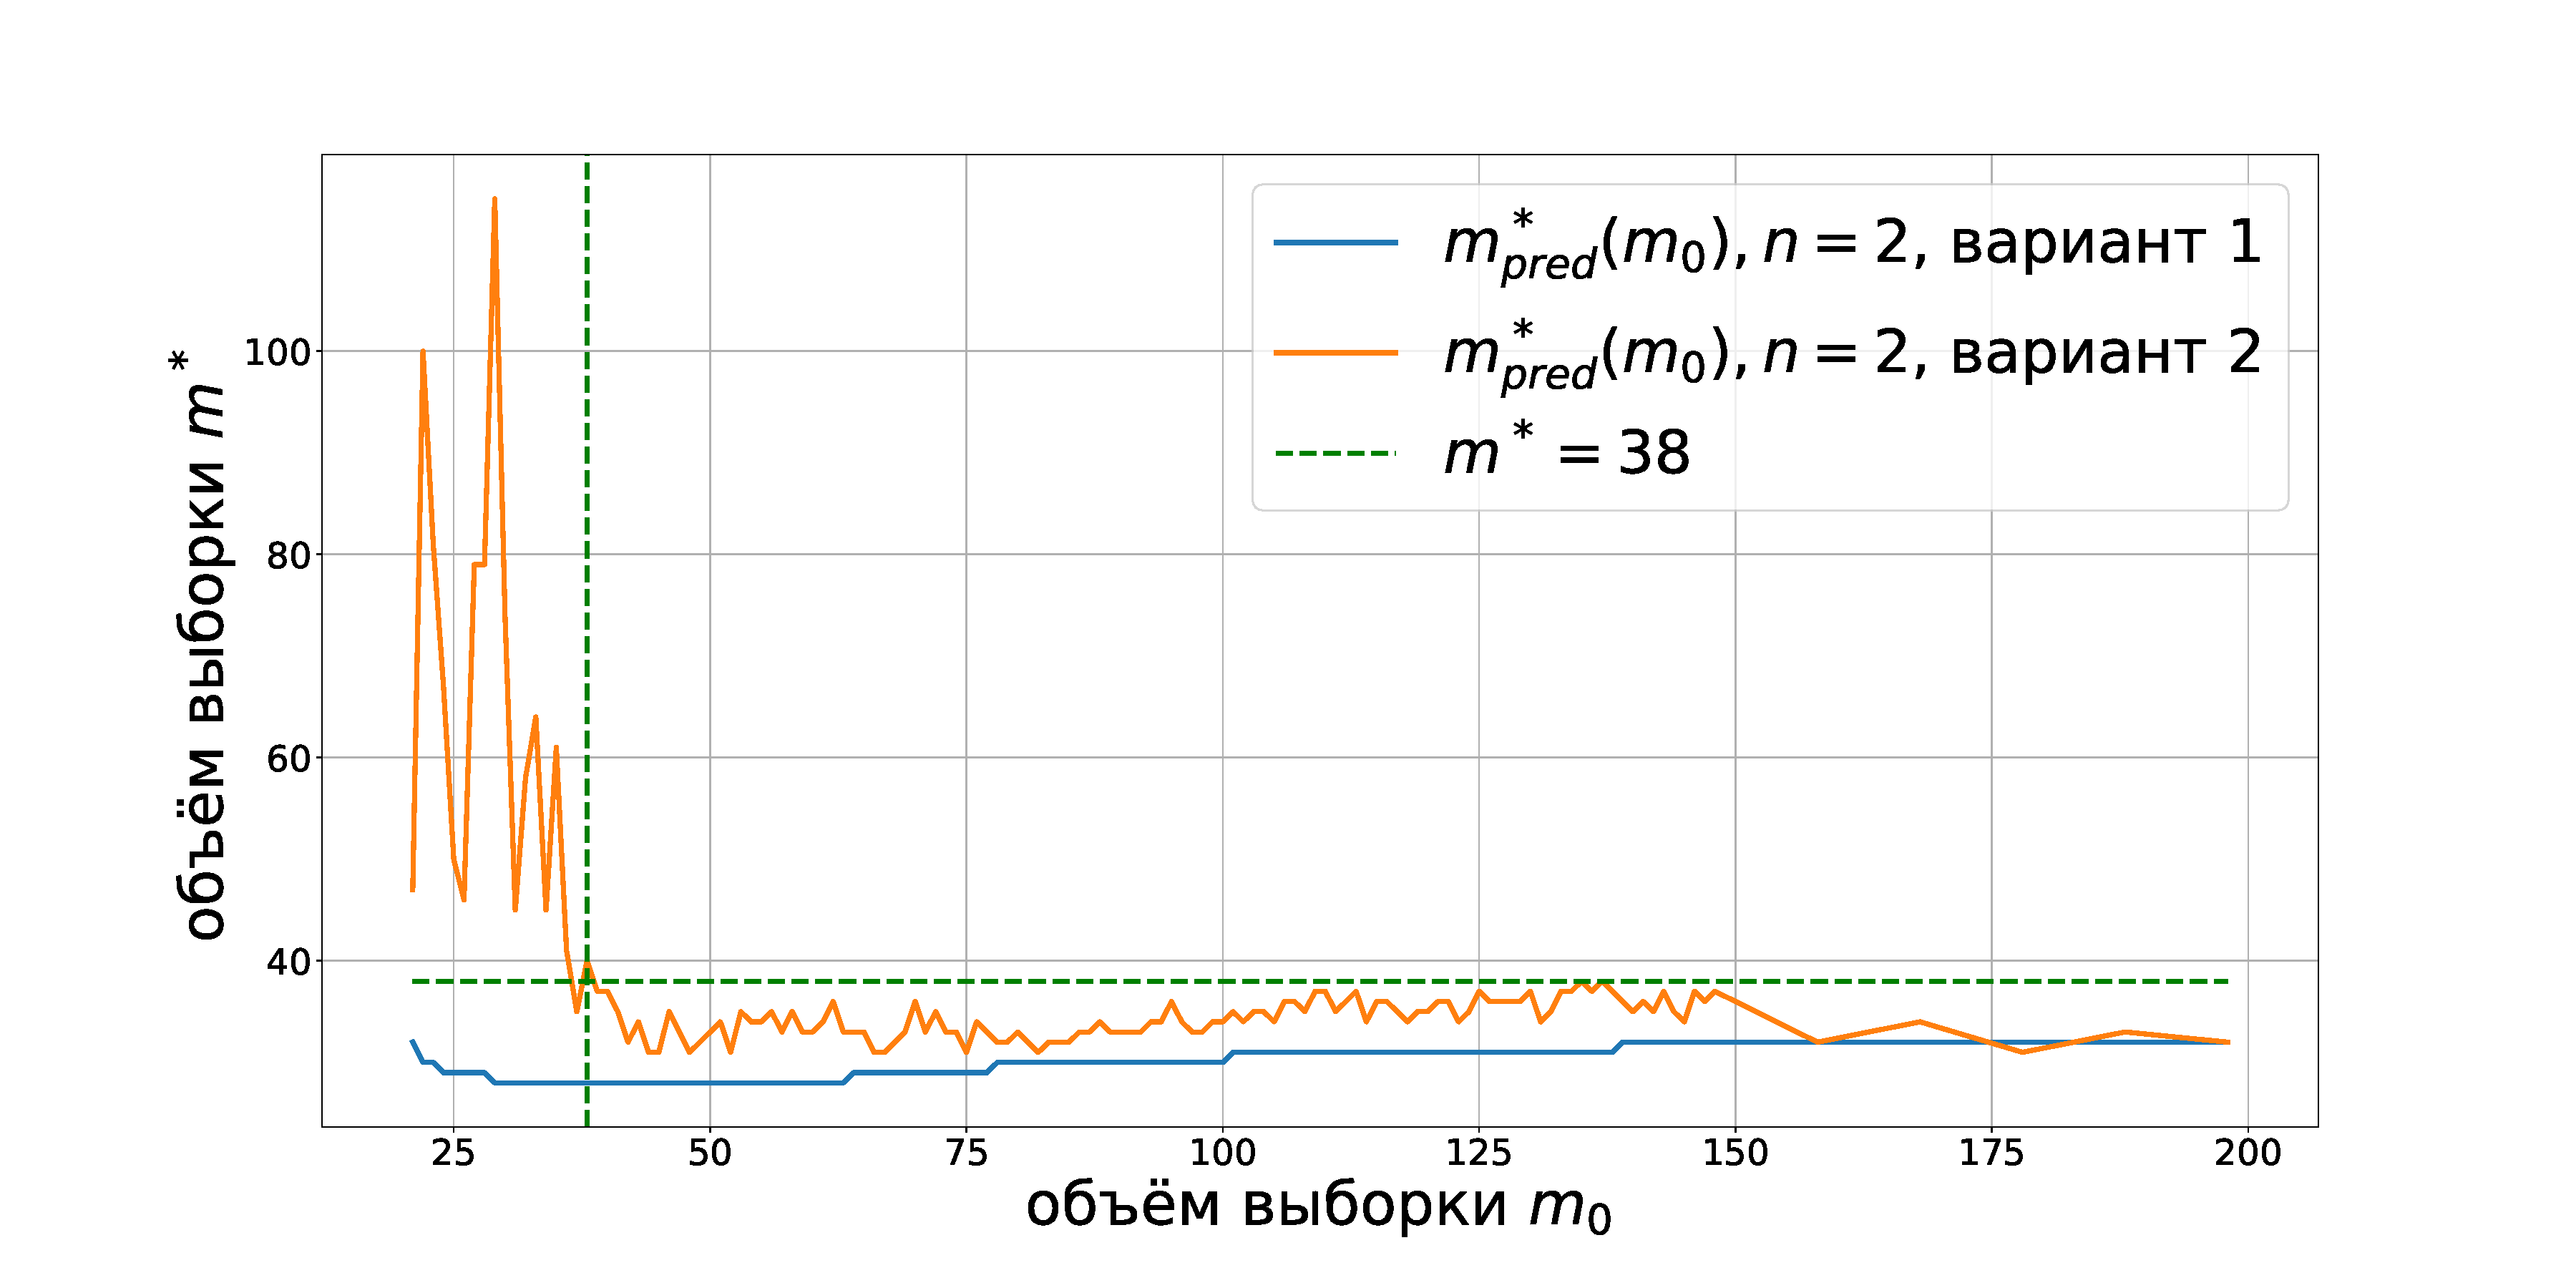
\includegraphics[width=0.5\textwidth]{../data/pics/nba_sample_MAPE_m_comparison_n2.pdf}}\\
\end{tabular}

\caption{Качество предсказания $e^{-S(m, n)}$ и $m^*$ в зависимости от объема обучающей выборки $m_0$ для выборки Nba}
\label{fig103}
\end{figure}

\end{frame}

\begin{frame}
\frametitle{Заключение}

\begin{itemize}
  \item Задача прогнозирования достаточного объема выборки сведена к задаче аппроксимации функции ошибок.
  \item Показана работоспособность предложенного метода на синтетических выборках, а также на выборках из UCI репозитория.
\end{itemize}

\end{frame}


\end{document}